\documentclass[LaM,english,noexaminfo,oneside]{sapthesis} % LaM for a Laurea Magistrale
\usepackage{microtype}
\usepackage{babel}
\usepackage[utf8]{inputenx}
\usepackage[hidelinks]{hyperref}
\usepackage{tabularx}
\usepackage{listings}
\usepackage{xcolor}
\usepackage{lipsum}
\usepackage{multirow}
\usepackage{bigstrut}
\usepackage{booktabs}
\usepackage{rotating}

\definecolor{ao}{rgb}{0.0, 0.5, 0.0}

\newcommand{\bluepill}{{\sc BluePill}}
\newcommand{\mynote}[1]{\marginpar{\color{red} #1}}

\lstset{
    language=C++,
    frame=tb, % draw a frame at the top and bottom of the code block
    tabsize=4, % tab space width
    showstringspaces=false, % don't mark spaces in strings
    numbers=left, % display line numbers on the left
    commentstyle=\color{ao}, % comment color
    keywordstyle=\color{blue}, % keyword color
    stringstyle=\color{red}, % string color
    basicstyle=\footnotesize\ttfamily,
    basewidth = {.48em}
}

\usepackage[backend=bibtex, maxbibnames=10]{biblatex}
\bibliography{biblio.bib}

%\setlength{\parindent}{4em}
\renewcommand{\baselinestretch}{1.5}

\hypersetup{pdftitle={My thesis},pdfauthor={Francesco Biccari}}
\title{BlueTracer: \\ a Robust API Tracer for Evasive Malware}
\author{Simone Nicchi}
\IDnumber{1705157}
\course{Master of Science}
\courseorganizer{Faculty of Information Engineering, Informatics and Statistics}
\AcademicYear{2017/2018}
\copyyear{2018}
\advisor{Prof. Camil Demetrescu}
\coadvisor{Dr. Daniele Cono D'Elia}
\coadvisor{Dr. Emilio Coppa}
\authoremail{nicchi.1705157@studenti.uniroma1.it}
\begin{document}
\frontmatter
\maketitle
\dedication{Ai miei genitori, che non hanno mai smesso di supportarmi}

\begingroup
\clearpage% Manually insert \clearpage
\let\clearpage\relax% Remove \clearpage functionality
\vspace*{-2cm}% Insert needed vertical retraction


\begin{abstract}

\iffalse     
With thousands of new malware samples surfacing every day, dy-
namic analysis techniques play a fundamental role in the automatic
characterization and detection of malicious behaviors that under-
mine the security of computing systems. And yet, often new threats
emerge that defeat automatic analysis, requiring them to be manu-
ally dissected by expert analysts. A significant fraction of strains
adopt however evasion techniques that hide their malicious behav-
ior if they are under the magnifying glass of an analyst, hindering
the analysis. We propose a methodology for hardening automatic
dynamic analysis techniques to make them more robust against
evasive malware. We build on binary instrumentation and we show
that more than 100 different anti-evasion techniques can be imple-
mented in terms of a minimal core of primitives to withstand com-
mon evasive behaviors. We discuss an embodiment of our approach
in the Pin dynamic binary instrumentation framework showing
how to construct a customizable stealthy sandbox that supports
remote debugging and dynamic taint analysis. We evaluate our
tool on a set of highly evasive malware samples and show how
taint analysis can help analysts to identify new evasive techniques;
countermeasures can then be incorporated into the analysis system
as part of a human-assisted feedback loop mechanism.
\fi

As a multitude of new malware instances arise every day, dynamic analysis techniques have assumed a key role in the detection and inspection of malicious software. One of the most adopted dynamic analysis strategies is function call monitoring, since the abstractions embodied by API calls and system calls can be used to comprehend the visible behaviour of the malware sample under analysis, regardless of any obfuscations made on its code. Function call monitoring is typically implemented by means of API hooking, i.e., the interception of function calls made available by dynamically linked libraries (DLL). However, all dynamic analyses techniques - including API hooking - have to face the adversarial behaviour of \textit{evasive malware} strains, which check if they are being executed in a hostile environment and conceal their malicious behaviour accordingly. Furthermore, the majority of API hooking techniques proposed to date in literature are detectable, as they are not equipped with cloaking methods to hide their presence from evasive malware.

We propose a robust library and system call tracer for Windows applications, specialized in evasive malware. To implement our tool, we used the Intel Pin dynamic instrumentation framework, which allows transparent injection of analysis code in a running binary program. In addition, our tool was integrated with BluePill, a stealthy execution framework developed at Sapienza University and Royal Holloway university, enabling BlueTracer to counteract a wide range of evasive techniques.

Our tracer is capable of tracing input parameters, output buffers and return values of a plethora of system calls (including Windows Native APIs) and library calls, as well as the occurrence of user-mode callbacks and Windows Asynchronous Procedure Calls. We first evaluated our tool on a set of benign applications performing a variety of tasks and exercising a large number of functions. Then, we validated it through the use of a popular security product aimed at assessing how stealthy a malware analysis system is with respect to a large body of public evasion techniques employed by real malware families seen in the wild.  

\end{abstract}
\endgroup

\tableofcontents

\mainmatter

% !TEX root = LMThesisNicchi.tex

\chapter{Introduction} \label{Intro}

\iffalse
Malwares are a threat

Dynamic analysis is favoured over static analysis

One dynamic analysis technique is API hooking/tracing

Malwares are also evasive

Problem: API hooking and tracing evasive samples

Solution BlueTracer
\fi

The term malicious software (\textit{malware} for short) describes any software specifically designed to bring harm to a computer system. Accurate and efficient analysis of malware is a compelling problem that is becoming increasingly important as hundreds of new malware strains arise every day in an ever-growing trend, while the economical damage for organizations keeps worsening~\cite{Cisco}.

To face this threat, professionals are typically aided by a range of automatic tools capable of analyzing and detecting malicious software. In particular, malware analysis can be carried out either statically or dynamically. Static analysis involves the inspection of the different code and data sections of a binary, but is often frustrated by obfuscation mechanisms and other countermeasures employed by malware authors. Dynamic analysis techniques dodge the problem by executing a malware sample and observing the actions it performs on the environment, and are better suited for dealing with large quantities of samples; these two factors have strongly favored the adoption of dynamic analyses in the security practice.

One of the most employed dynamic analysis techniques is function call monitoring. Generally speaking, a function is made up of code that carries out a particular task, such as creating a file or printing a message. A property that makes functions particularly valuable from a program analysis perspective is that they can abstract implementation details - especially in the case of library and system calls - providing a semantically richer representation of some functionality. Consider for instance a sorting function: details of the underlying algorithm might not be important as long as one knows that the function sorts an input list. In the context of dynamic analysis, the abstractions embodied by API calls and system calls are incredibly helpful since they can be used to grasp the visible behavior of the sample under analysis, regardless of any obfuscations made on its code.

The most popular technique used for function call monitoring in dynamic malware analysis is API hooking, i.e., the interception of function calls provided by dynamically linked libraries (DLL). The idea is to alter execution so that for each call in the sample, besides the function of interest, a hooking function is called, too. Such function is in charge of performing the desired analysis, which may require for instance logging the invocation on a file or analyzing its parameters.

A problem that nearly all dynamic analyses - including API hooking - have to face is adversarial behavior from \textit{evasive malware}, i.e., malware that actively checks whether it is being executed in a hostile environment, such as a well-known sandbox solution for dynamic analysis. In that case, an evasive sample conceals its harmful behavior to avoid detection, for instance by executing an exit sequence. Evasive techniques are frequently adopted by modern malware. According to a March 2018 Symantec Internet Security Report, 18\% of recently observed new samples are aware of hardware virtualization solutions used also for malware analysis \cite{Symantec}. To make matters worse, most API hooking techniques proposed to date in literature are easily detectable by malware, and not coupled with mechanisms to hide their presence from evasive malware.

\paragraph{Contributions.}The core contribution of my thesis is the design and implementation of BlueTracer, a robust library and system call tracer for Windows programs specialized in evasive malware.

BlueTracer is based on the Intel Pin~\cite{Luk05} dynamic binary instrumentation framework, which allows for transparently injecting analysis code in a binary program as it executes. BlueTracer can effectively counteract a large variety of evasive techniques due to its integration with BluePill~\cite{BluePill}, a stealthy execution framework being developed at Sapienza University and Royal Holloway University of London that allows the simulation of the original execution environment a particular malware sample was designed for, and conceals any analysis artifacts or setup details that might set off evasion \cite{BluePill}.

BlueTracer can trace input parameters, output buffers and return values of an extremely wide range of system calls (including Windows Native APIs that are invoked directly via special CPU instructions in more advanced malware) and library calls. Moreover, it also supports the tracing of user-mode callbacks and Windows Asynchronous Procedure Calls. 

The heterogeneity of Windows libraries used in malware and the lack of well-structured documentation for their prototypes and input/output parameters posed a significant implementation challenge, which BlueTracer addresses by leveling out and integrating reliable external sources (two industry projects: Dr. Memory \cite{DrMemory} and CISCO PyREBox \cite{Pyrebox}) that account for more than 17,000 existing function prototypes. An important engineering effort was also required to make best use of Intel Pin’s capabilities with respect to run-time CPU and memory costs, as well as to address some inherent limitations that emerged on the field.

We first validated BlueTracer on benign applications exercising a large number of functions, and then on a popular security product used for assessing how stealthy a malware analysis system is against a large body of public evasion techniques used in the wild. The obtained results suggested that BlueTracer can be very effective in tracing a malware sample's activities while remaining undetected. 
\iffalse
I then analyzed a set of highly evasive samples collected by Joe Security, the proclaimed technology leader for the analysis of evasive malware, as they feature exotic evasions that most analysis products have struggled to deal with. The logs collected by BlueTracer reveal behaviors consistent with the analysis reports authored by Joe Security, suggesting that BlueTracer can be very effective in tracing a malware sample's activities while remaining undetected. 
\fi               

\paragraph{Structure of the Thesis.}
The remaining part of this thesis is structured as follows.
Chapter \ref{background} describes the major \textit{API hooking} techniques present in literature, outlining their stengths and weaknesses, especially from a detection point of view. It also introduces the concept of Dynamic Binary Instrumentation (DBI), which constitutes BlueTracer's core.
Chapter \ref{implementation} focuses on the implementation of the tool, on its structure and the design choices which were made during its development.
Chapter \ref{conclusion} illustrates the experimental results and assesses the tool's effectiveness.
Finally, we present concluding remarks in Chapter 5, together with possible future developments.

% !TEX root = LMThesisNicchi.tex

\chapter{Background} \label{background}

In literature there are many different implementations of API hooking. The objective of this chapter is to provide an outline of the various approaches utilized to hook functions in DLLs, outlining the benefits and the limitations of each technique, with a strong focus on their detection by malicious software. In particular, the focus will be on user space API hooking of \texttt{Win32} binaries, since this is BlueTracer's current field of application. Obviously, as it is the norm in malware analysis, it also assumed that the program under study is only available in binary form.

Depending on their underlying implementation, API hooking techniques can be divided in three broad categories: \textbf{Binary Rewriting}, \textbf{Virtul Machine Introspection (VMI)} and \textbf{Dynamic Binary Instrumentation (DBI)}.   

\section{Binary Rewriting}

Binary rewriting-based hooking involves inserting hooks at the API entries, via one of the following two approaches:
\begin{enumerate}
\item Redirecting all \texttt{call} instructions so that the hook is called instead of the original function.
\item Rewriting the function of interest such that, before its invocation, the hook is executed. 
\end{enumerate} 

In both cases the hook function gains access to all the arguments present on the stack, thus being able to carry out all the required analysis operations.

The main techniques which use the first approach are \textit{Import Address Table (IAT) Patching}, \textit{Export Address Table (EAT) patching} and \textit{Proxy DLL}. On the other hand, the most significant techniques which use the second approach are \textit{inline hooking} and \textit{debugger-based hooking} (\textit{Figure~\ref{HookTech}}).



\begin{figure}[h]
\centering
\hspace*{-3em}
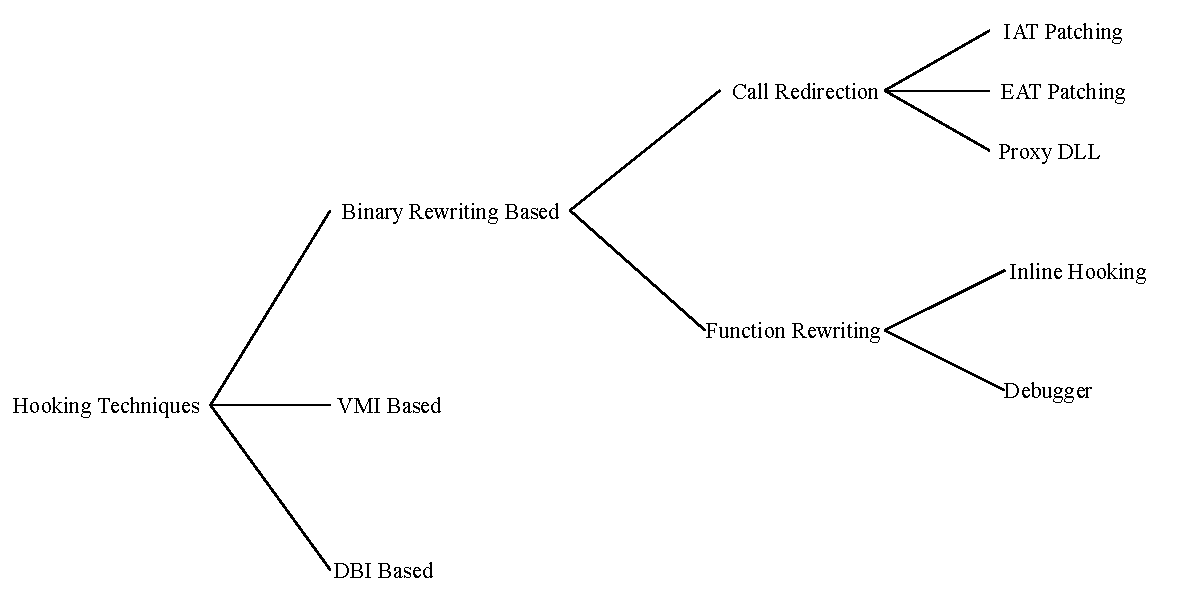
\includegraphics[scale=0.8]{Figures/API-hooking-3.pdf}
\caption{\textit{API hooking techniques classification}}
\label{HookTech}
\end{figure}

\subsection{Import Address Table Patching}

In the header of every Portable Executable (PE) file there is an Import Address Table (IAT) for every dynamic-link library (DLL) that is included by the executable \cite{Berdajs:2010:EAU:1815744.1815746} (\textit{Figure~\ref{IAT}}). This table is utilized to indicate the location of DLL-imported functions in virtual memory and is filled by the Windows loader with the actual function memory addresses after the executable is loaded in memory.

\begin{figure}[h]
\centering
\hspace*{-3em}
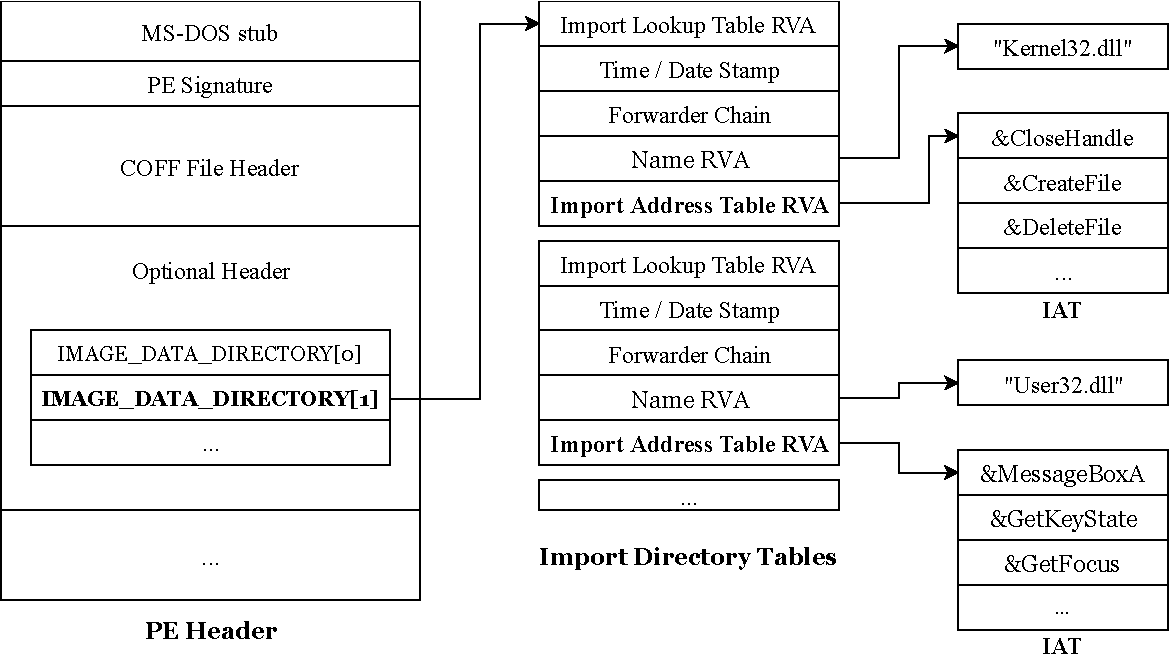
\includegraphics[scale=0.8]{Figures/IAT-3.pdf}
\caption{\textit{IAT in PE header}}
\label{IAT}
\end{figure}

The idea is to overwrite the original pointer to an imported API function so that, instead of pointing to the original API, it will point to a different function.

\newpage

Despite being extremely simple to implement, IAT patching suffers from a couple of disadvantages, which significantly limit its use in practice:
\begin{itemize}
    \item It is incredibly easy to detect by simply examining the entries of the IAT and checking whether or not each address falls inside the memory range of the DLL that should contain the function \cite{HookingDetection}.
    \item It is ineffective when function pointers are acquired dynamically, e.g., via \texttt{LoadLibrary} and \texttt{GetProcAddress} \cite{Buescher:2011:BIS:2186328.2186347}.
\end{itemize}

\subsection{Export Address Table Patching}

Export Address Table (EAT) patching is similar to IAT patching, with the difference that DLL export address tables are patched instead. The export address table (EAT) contains the name of every function exported by the DLL together with the relative virtual address (RVA) where the function can be found, which is relative to the DLL base address when loaded in memory. To hook an API function via EAT patching all that is needed is to overwrite the corresponding address in the table with the address of another function.

EAT patching produces similar results to the ones obtained through IAT patching, but, unlike IAT patching, the created hooks are global, i.e., they affect every program which utilizes the altered DLL \cite{Berdajs:2010:EAU:1815744.1815746}.

However, in a similar manner to what occurs for IAT patching, it can be easily detected by simply examining the entries of the EAT and checking whether or not each RVA, when added to the DLL base address, falls within the DLL memory range \cite{Stuttard:2014:ADC:2616217}.

\subsection{Proxy DLL}

In the Proxy DLL approach to hooking, also known as Trojan DLL, the DLL containing the functions to be hooked is replaced with another one having an identical name and exporting all the symbols of the original DLL \cite{CodeProjectHooking}. In addition to calling the original functions so that they can carry out their tasks, the Proxy DLL may also make available different implementations for the hooked functions \cite{Berdajs:2010:EAU:1815744.1815746}.

Even though a Proxy DLL is trivial to implement, it is also extremely easy to detect since the original DLL is substituted with another file, which is very likely to have a different size. Moreover, checksums could be employed to detect the presence of a Trojan DLL.


\subsection{Inline Hooking}

In \textit{inline hooking} the API to be hooked has its initial instructions (at least the first 5 bytes) overwritten with an unconditional jump to a replacement function. In order to ensure that the API's original functionality is not lost due to the modification of its entry point, a \textit{trampoline function} is created, consisting of a copy of the overwritten instructions and an unconditional jump back to the unaltered portion of the original function. As a result of this, the replacement function can invoke the original function by calling the trampoline, after performing all the desired analysis operations \cite{Berdajs:2010:EAU:1815744.1815746}.
\textit{Figure~\ref{Inlined}} illustrates a program's execution flow before and after the use of \textit{inline hooking}.

\begin{figure}[h]
\centering
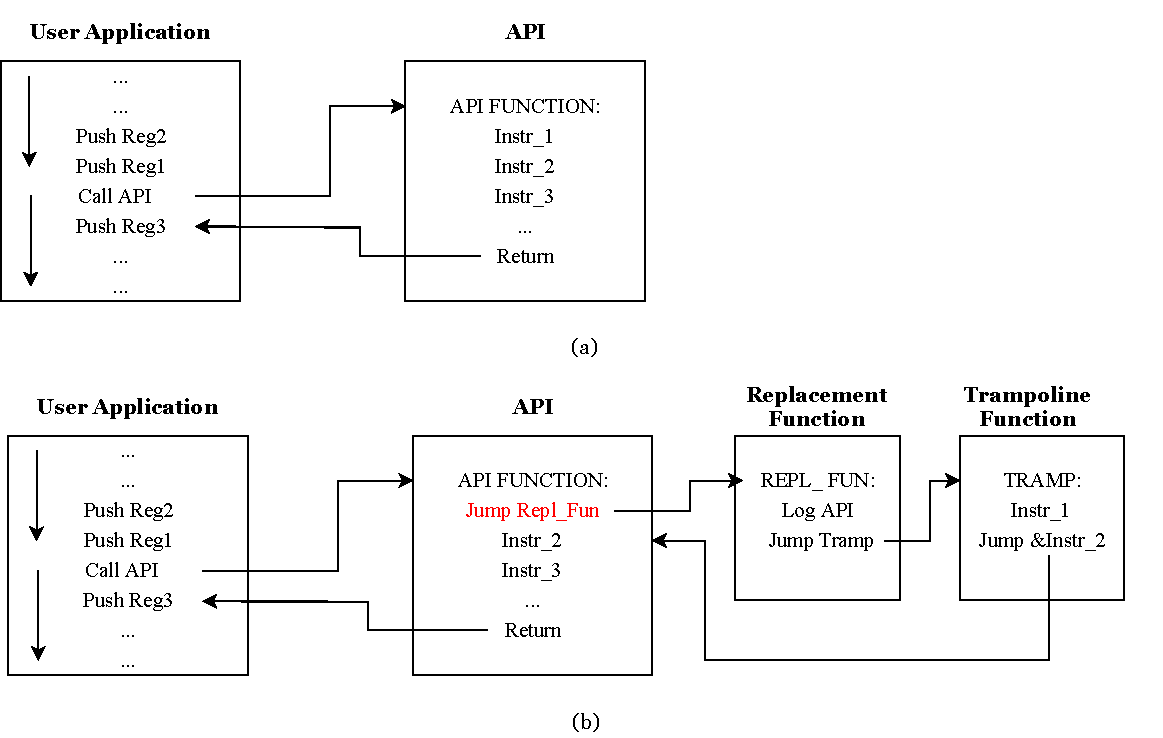
\includegraphics[scale=0.8]{Figures/Inline.pdf}
\caption{\textit{(a) Ordinary API call execution flow \\
				  (b) API call with inline hooking}}
\label{Inlined}
\end{figure}

\textit{Inline Hooking}, which was made famous by its employment  in the Microsoft \textit{Detours} Windows API hooking library, is one of the most used API hooking techniques since it offers a number of advantages:
\begin{itemize}
\item It is fast and efficient.
\item It can be utilized to hook any code, not just operating systems APIs, but also programmer defined functions \cite{Rootkit}. 
\item Unlike IAT patching, the type of command used to call the function does not matter, meaning that the hooking will be effective regardless of the fact that a function is called using the IAT or using \texttt{LoadLibrary} together with \texttt{GetProcAddress}.
\end{itemize} 

Unfortunately though, \textit{inline hooking} is also affected by some limitations:

\begin{itemize}
\item Can be easily detected, for instance by comparing the code section of system libraries in memory with a matching original copy loaded from the file system to detect library modifications \cite{Buescher:2011:BIS:2186328.2186347} or by searching API entry points for specific patterns (e.g., presence of \texttt{jmp} instructions) \cite{HookingDetection}.
\item It needs additional modifications in the case where the function's entry points includes specific instructions, like ones which contain relative memory addresses. In fact, such instructions cannot be executed from a trampoline as the trampoline is located in a different memory location than the one of the original program code \cite{Berdajs:2010:EAU:1815744.1815746}.
\end{itemize}

\subsection{Debugger-Based Hooking} \label{Debugger}

Hooking through the use of a debugger is realized by instructing the debugger to position a breakpoint at the entry point of the target API function. The placement of a breakpoint involves overwriting the initial instructions of the target API functions with CPU specific instructions, like \texttt{INT 3} for \texttt{IA-32}. These lead the CPU to throw a debug exception in case they are pointed by the current instruction pointer (IP). The exception is then intercepted by the debugger, which is able to deduce the API which is being called by the application from the address at which the exception took place \cite{HookingDetection}. Moreover, the debugger also has total control over the memory contents and the CPU state of the process being debugged.

Contrarily to inline hooking, a debugger can be used to hook functions whose entry points include instructions containing relative addresses \cite{Berdajs:2010:EAU:1815744.1815746}.

On the other hand, a debugger is much easier to detect. In fact, there exist specific Windows APIs whose purpose is to find out whether or not the current process is being debugged. For example, \texttt{IsDebuggerPresent} allows to determine if the calling process is running under a debugger, while \texttt{CheckRemoteDebuggerPresent} checks for the presence of a debugger in a separate process. 
In addition, the \texttt{INT 3} instruction in an API entry point immediately gives away the debugger's presence \cite{HookingDetection}.



\section{Virtual Machine Introspection}

Hooking based on Virtual Machine Introspection (VMI) relies on the idea of executing the target program in an emulated environment, typically with QEMU being used as virtual machine monitor (VMM). Function calls are monitored by comparing the virtual processor's instruction pointer with the RVAs of DLLs' exported functions when added to the DLL base address. Function arguments are also monitored and this is done by providing them to callback routines, which perform the appropriate tracking operations.

In theory, a PC emulator allows to have functionalities similar to the ones of a debugger, i.e., the code being monitored can be stopped at any arbitrary point during its execution, allowing its registers and virtual memory to be inspected, with the added advantage of not being subject to the aforementioned issues related to breakpoints.
Moreover, VMI-based hooking is harder to detect with respect to the previously illustrated hooking techniques, since emulation is utilized to execute an unknown binary with a complete operating system in software, without the sample being never ran directly on the processor \cite{Bayer2005TTAnalyzeA}.

The significant drawback of VMI-based hooking is that it incurs in the \textit{semantic gap} problem, i.e., the issue of deducing high-level information from the raw system information by making sense of the CPU state and memory contents \cite{Egele:2008:SAD:2089125.2089126}. VMI-based hooking tools
might need an in-depth knowledge of kernel data structures or other details at low-level, which could constitute a complication when dealing with proprietary operating systems. For this reason, as of right now, VMI is not as effective in practice as a traditional debugger when investigating a sample.


\section{Dynamic Binary Instrumentation} \label{DBI}

\iffalse
- Program analysis: source vs binary. As opposed to source analysis, in which ..., in binary analysis the idea is blablabla. The employed technique here is instrumentation.
- Instrumentation is blablabla. It can be either static or dynamic, where in both cases it is mandatory blablabla.
- Dynamic is better because blabla.
- Its main drawback is performance but recent frameworks blablabla
\fi

Instrumentation is commonly referred to as the act of adding extra analysis code to a program. There are two main instrumentation techniques being employed in dynamic binary analysis, where the main difference is constituted by when the instrumentation process takes place:

\begin{itemize}
\item \textit{Static Binary Instrumentation}, which takes place before the application is executed and involves the rewriting of object code or executable code.
\item \textit{Dynamic Binary Instrumentation} (DBI), 	which happens at run-time. The analysis code can be injected by a specific program attached to the target process or by an external process \cite{Nethercote2004CI}. 
\end{itemize}   

Dynamic Binary Instrumentation (DBI) is, therefore, a dynamic binary analysis technique in which the behavior of an application is inspected at run-time via the injection of analysis code. Such code, after being injected, executes as a component of the ordinary instruction flow, allowing to learn information about the behavior and the state of a sample at different points during its execution \cite{DBI}. Typically, DBI tools make use of a Just In Time (JIT) compiler to instrument the binary under analysis at run-time, the purpose of which is to translate \texttt{x86} code into an intermediate representation \cite{polino_arancino_2017}.

DBI, conversely from static binary instrumentation does not need any preprocessing of the program to be analyzed. This is what makes it more appealing for developers for profiling and tracing purposes. On top of that, DBI can be utilized for any program while static techniques are restricted in the code they can instrument, e.g., they cannot employed for code that is dynamically generated \cite{6658603}. The main drawback of DBI is that the instrumentation cost is encountered at run time, leading to performance degradation. However, in recent years, this issue has been mitigated by the introduction of generic DBI frameworks, which are accurately optimized to minimize the execution overhead \cite{Nethercote2004CI}.

In DBI-based hooking, the idea is to use DBI with the objective of learning information at run-time relative to which APIs are called by the sample being analyzed and, possibly, with which arguments and return values. 

There indeed exist DBI-based API tracing tools that rely on the previously illustrated idea, namely \textit{drstrace} and \textit{drltrace}, which are both built on top of the DynamoRIO \cite{DynamoRIO} DBI framework. In particular, \textit{drstrace} is a system call tracer for Windows, while \textit{drltrace} is an API calls tracer for both Windows and Linux applications. They both produce a textual log, in which the invoked APIs are recorded, together with their argument values and return values.

In order to evaluate the effectiveness of such tools in the context of evasive malware analysis, a series of experiments involving them was carried out. In particular, both tools were employed to analyze 1000 random samples from the Arancino\footnote{Arancino is a dynamic protection framework aimed at providing protection from anti-instrumentation attacks \cite{polino_arancino_2017}} dataset of malware samples (about 20\% of the total). Each malware sample was ran for 5 minutes in a VirtualBox environment with Windows 7 \texttt{x86} SP1 as the guest operating system. The analysis of the resulting logs showed that both tools possess critical shortcomings when analysing evasive malware. In particular: 

\begin{itemize}
\item They are not equipped with any mechanism aimed at cloaking the execution environment in order to prevent a malicious sample from detecting the DBI.
\item They are limited in the amount of information recorded relative to the traced APIs. This applies particularly to \textit{drltace}, which, unlike \textit{drstrace}, does not log return values and output values for arguments, in addition to not providing a mechanism for translating enumerations' constants to the appropriate name. Furthermore, both tools do not take into consideration Windows callbacks and asynchronous procedure calls (APC).
\end{itemize}

This highlights how the current DBI-based methods are lacking when having to deal with the dynamic analysis of evasive malware and that there is much room for improvement in this area.

\section{Conclusion}

In this chapter we showed how the state of the art API hooking techniques suffer from a number of remarkable shortcomings, especially when dealing with evasive malware. In fact, binary rewriting-based hooking techniques are all easily detectable, while VMI, although harder to uncover, is affected by the \textit{semantic gap problem}. Finally, existing DBI-based API tracing tools are not accompanied by adequate cloaking mechanisms and are limited in the amount of logged information. The aforementioned issues indicate that there is a need for a robust API tracer, specialized in the analysis of evasive malware and with extensive logging capabilities. This is the rationale at the heart of BlueTracer. 
\cleardoublepage
\phantomsection % Give this command only if hyperref is loaded
% !TEX root = LMThesisNicchi.tex

\chapter{Architecture and Implementation}
In this chapter we discuss the implementation of BlueTracer, providing a detailed account on how the tool is organized, on the design choices which were made during its development process, on how encountered challenges were dealt with and on the decisions which were taken to improve performance.

\section{Overview}

BlueTracer\mynote{This section requires significant extensions}, being a part of Blue Pill, is also implemented using Pin, a dynamic binary instrumentation framework by Intel, which is vastly utilized for program analysis, testing of software and in the security field. The version of Pin used for the development of the tool is 3.5, in order to benefit from the notable improvements, both in terms of execution speed and offered features, which were introduced going from the 2.14 release to the 3.x series. Pin comes with its own OS-agnostic and compiler-agnostic runtime, called PinCRT. PinCRT exposes three layers: a generic operating system interface providing basic OS services (e.g. process and thread control), together with C and C++03 (without RTTI) runtime layers, for writing instrumentation and analysis routines \cite{Pin}.   

BlueTracer has been organized primarily taking into account the rich set of APIs offered by Pin, which have led to the decision to split the tool in three parts: the first aimed at \textbf{native APIs tracing}, the second for \textbf{APIs tracing} and the last focused on \textbf{callbacks and APCs tracing} (\textit{Figure 3.1}). In particular, the tracing of native APIs also employs a different source of API information (\textit{Dr. Memory}'s system call data) than the ones utilized for tracing APIs (\textit{drltrace}'s configuration file or the information extracted from \textit{PyREbox}'s database).

This chapter will begin by describing how multi-threading was addressed in the tool, as this is central to all its components. Then, the implementation of each one of three aforementioned parts will be discussed in detail. 
\iffalse
Finally, all the configuration options of the tool will be explained.          
\fi

\begin{figure}[h]
\centering
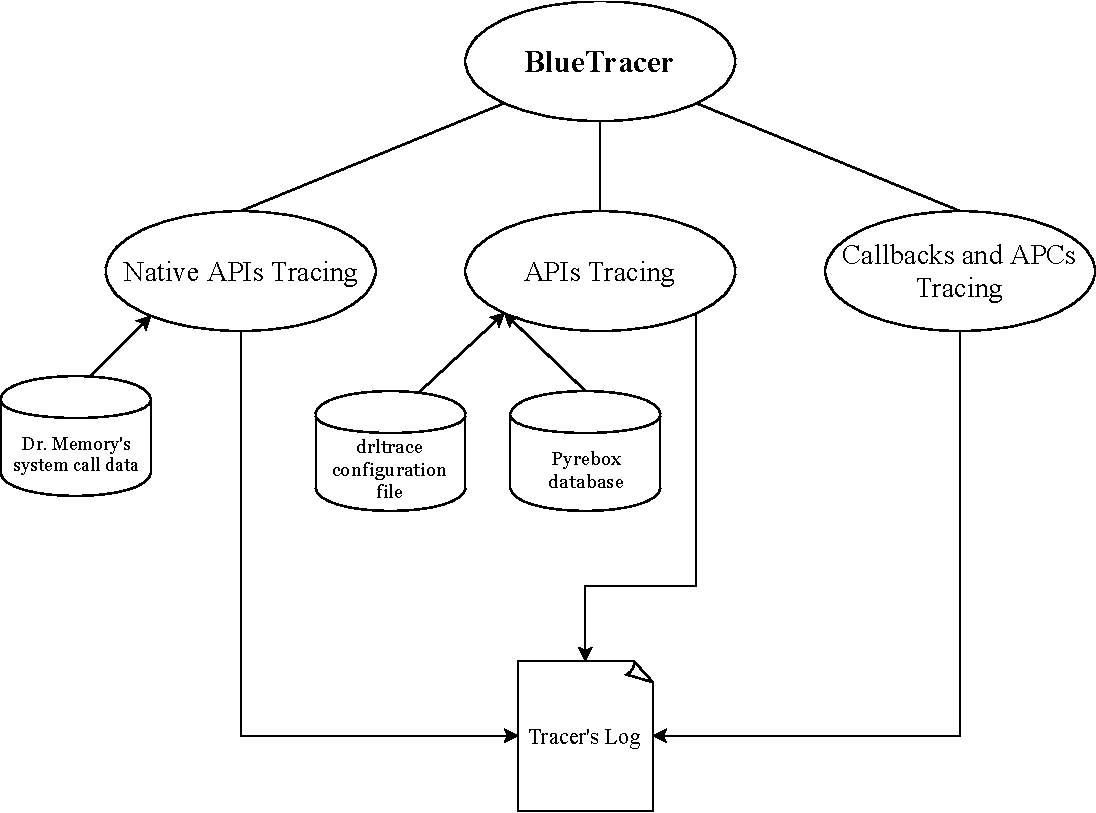
\includegraphics[width=0.85\textwidth]{Figures/BlueTracer.pdf}
\caption{\textit{BlueTracer's high level structure}}
\end{figure}

\section{Thread Management}

Since the samples under analysis are typically multithreaded applications, let us go through the mechanisms exposed by Pin to manage threads and how those were employed in the implementation of the tool.

Pin assigns to each thread an ID, a small number beginning at 0
which is not the same as the operating system thread ID. A way to obtain such ID is by using as analysis routine argument \texttt{IARG\_THREAD\_ID}, which passes the thread ID assigned by Pin for the calling thread. This ID is typically used as an index of an array of thread data.
In fact, the Pin API makes available an efficient thread local storage (TLS). In order to utilize it, it is first required to allocate a new TLS key via \texttt{PIN\_CreateThreadDataKey}, which can optionally take as input a pointer to a destructor function. After that, any thread of the process can use the TLS key, in addition to its Pin-specific thread ID, to store (\texttt{PIN\_SetThreadData}) and retrieve (\texttt{PIN\_GetThreadData}) values in its own slot. The starting value relative to the key in every thread is \texttt{NULL}.
Pin makes also available call-backs when each thread starts (registered with \texttt{PIN\_AddThreadStartFunction}) and ends (registered with \texttt{PIN\_AddThreadFiniFunction}). This is typically where thread local data is allocated, manipulated and stored in a thread's local storage\cite{Pin}.

In BlueTracer, each TLS slot stores a \texttt{struct} of the type \texttt{bluepill\_tls} (\textit{Listing 3.1}) for every thread. Such \texttt{struct} is dynamically allocated every time a thread starts in the \texttt{OnThreadStart} callback function and is consequently deallocated in the \texttt{onThreadFini} function when the thread ends.

\vspace{0.5cm}
\begin{lstlisting}[caption={Thread Local Data},captionpos=b]
typedef struct {
 ...
 syscall_tracer* syscallEntry;     // Pointer to NTAPI entry
 vector<stackEntry>* shadowStack;  // Shadow stack
 uint call_number;             	   // Calls counter							
 
 buf_info_t* buffer;		   	   // Buffer for writing to file				 
 FILE* OutFile;                    // Output file pointer
 
 // Pointer to function for opening file/writing to file	
 void(*file_write)(THREADID, buf_info_t*, FILE*, const char*, 	...);
 
 ...
} bluepill_tls;
\end{lstlisting}

Since the first three fields of the above \texttt{struct} (lines 3-5) are employed when tracing native APIs and APIs, they will be discussed in detail later in the chapter. Now let us focus on the remaining fields, which are used by BlueTracer to write the traced information in the appropriate log files. 

\subsection{Log Files and Multithreading}

In BlueTracer, the traced data is written to a binary file, one for every thread. The default naming convention used for the tracer's log files is \texttt{Traced.[OS Process ID].[Pin-specific Thread ID]}, similarly to the one Blue Pill employs in its own log files, with the user being able to change \texttt{Traced} with a name of its choice in the configuration file. 

When writing data to file, each thread invokes the \texttt{file\_write} function, whose pointer is located in the instance of the \texttt{bluepill\_tls} struct associated to the thread (line 11 of \textit{Listing 3.1}). However, such data, which follows the same format of strings used by \texttt{fprintf}, is not directly written to file. Instead, an intermediate 8 kB buffer is used (line 7 of \textit{Listing 3.1}): only when the buffer is full (or when the amount of data to be written does not fit the buffer) file writing actually occurs. The choice of using a buffer was made as an attempt to improve performance, as it allows the aggregation of small write operations into a block size that is more efficient for the disk subsystem.

A problem which was encountered when trying to conjugate file management and multithreading is that there exists a known isolation issue affecting Pin on Windows. Specifically, it is possible for a deadlock to take place if a file is opened in a callback in the context of multithreaded applications. As a result of this issue, it is not possible to open the tracer's log file in the \texttt{OnThreadStart} callback. Pin's manual proposes to circumvent the problem by opening the file in the \texttt{main} and tagging the data with the thread ID \cite{Pin}. However, this conflicts with the idea of having one file for each thread.

In order to bypass this limitation of the Pin's framework, the following strategy was employed:
\begin{enumerate}
\item When initializing the thread local data in \texttt{OnThreadStart}, \texttt{file\_write} is set to point to a function named \texttt{file\_open}.
\item The first time a thread attempts to write data to file \texttt{file\_open} is invoked.
\item \texttt{file\_open} carries out the following actions:
\begin{enumerate}
\item Opens the tracer's log file (this is safe since the file is not opened in a callback)
\item Sets the obtained file pointer in the thread local data (line 8 of \textit{Listing 3.1})
\item Adds the data to be written in the buffer (which is eventually written to file if the buffer is too small to hold it)
\item Sets \texttt{file\_write} to point to \texttt{buf\_write}, a function which is in charge of just writing data to the buffer and to file.
\end{enumerate}
\item As a result of this, when the thread attempts to write to file again, \texttt{buf\_write} is invoked, thus allowing the thread to just write to file without going through opening the file again.   
\end{enumerate}   

\section{Native APIs Tracing}
\iffalse
Talk about log structure when talking about how arguments are printed
\fi

Windows Native APIs are employed to call operating system services in kernel mode in a controlled way.  
In fact, all core Windows components, which possess direct access to hardware and services in charge of handling the computer's resources (e.g. memory), operate in kernel mode. This means that, every time a user mode application desires to carry out certain actions, like for instance starting a thread or allocating virtual memory, they must rely on kernel mode  services. The Windows Native API corresponds to the system call interface of standard monolithic operating systems, such as the majority of UNIX-like systems, with the difference that in the latter case the system call interface is documented and can be utilized directly by applications. Instead, due to Windows' architecture, Windows Native APIs are concealed to the programmer by the higher level Windows (\texttt{Win32}) APIs \cite{NTAPI1}. User mode Windows Native APIs, which are identified by their \texttt{Nt} prefix and are exported by \texttt{ntdll}, have caught the attention of malware writers since they are seen as a way of bypassing the documented APIs with the objective of performing a series of actions without being discovered \cite{NTAPI2}. For this reason it is a good idea to also trace them, in addition to the ordinary Windows APIs.  

Pin provides a set of APIs aimed at assisting the extraction of information relative to the system calls made by the pinned application, also including information relative to Windows Native APIs. In particular, in Blue Pill (and consequently in BlueTracer) \texttt{PIN\_AddSyscallEntryFunction} and  \texttt{PIN\_AddSyscallExitFunction} were used for this purpose. In fact, these allow to register notification functions which are called immediately before and after the execution of a system call \cite{Pin}. In BlueTracer, the function in charge of gathering Native API information before execution is \texttt{TraceSysCallEntry} while the one responsible for collecting Native API information after execution is \texttt{TraceSysCallExit}. They have been both been embedded in Blue Pill's notification functions and their overall structure is detailed in \textit{Figure 3.2}.
\\
\begin{figure}[h]
\centering
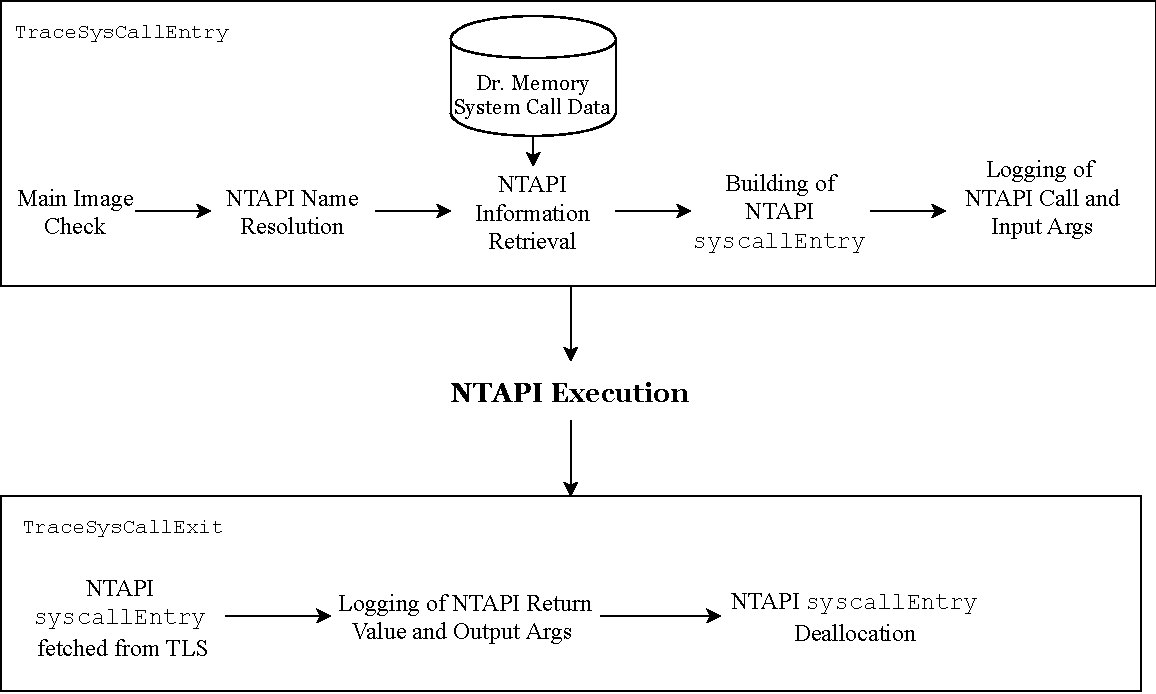
\includegraphics[scale=0.75]{Figures/NTAPITracing.pdf}
\caption{\textit{Native APIs Tracing Workflow}}
\end{figure}
\\
Following \textit{Figure 3.2}, let us now thoroughly analyze the main steps which take place when Native APIs are traced.

\subsection{Main Image Check}
In order to filter the logged information relative to Native APIs, BlueTracer allows the analyst to decide, through the use of a boolean parameter (\texttt{MainImage}) in the configuration file, whether or not only Native APIs called invoked directly from the main executable of the pinned application should be traced. Therefore, as it can be seen in \textit{Figure 3.2}, the first thing which is done in \texttt{TraceSysCallEntry}, assuming that the \texttt{MainImage} configuration parameter has been set to \texttt{true}, is to determine if the Native API call is taking place directly from the main executable.

To this end, Pin's \texttt{IMG} APIs are employed, where in Pin an \texttt{IMG} represents all the data structures relative to binaries and shared libraries \cite{Pin}. Specifically, in Blue Pill, \texttt{IMG\_AddInstrumentFunction} is utilized to register a callback which is invoked each time an image is loaded. Inside such callback, which takes as one of the input parameters the \texttt{IMG} object representing the image being loaded, the following steps are taken:
\begin{enumerate}
\item \texttt{IMG\_IsMainExecutable} is employed to determine if the image being loaded is the main executable of the pinned application.
\item If this is the case, \texttt{IMG\_HighAddress} and \texttt{IMG\_LowAddress} are invoked. These two APIs return the highest address and the lowest address respectively of any code or data loaded by the image corresponding the the \texttt{IMG} object they take as input. By employing these APIs is therefore possible to determine the address range relative to the main executable. 
\end{enumerate}  

Having obtained the main executable address range in this way, it is then employed in \texttt{TraceSysCallEntry} to learn if the Native API call is occuring directly from the main image. Internally, before entering kernel mode every Native API executes some common code, i.e. each Native API stores its ordinal in the \texttt{eax} register and invokes \texttt{KiFastSystemCall}, where the \texttt{sysenter} instruction is used to actually enter kernel mode. When \texttt{sysenter} is executed, the kernel obtains the ordinal number from \texttt{eax} and utilizes it to call the corresponding function, prior to going back to user mode \cite{MalwareTech}.

In Pin, the Native API is intercepted right before \texttt{sysenter} is executed. This could be inferred by the fact that, in \texttt{TraceSysCallEntry}, the instruction pointer (obtainable via the \texttt{PIN\_GetContextReg} API) contains \texttt{sysenter}'s address. In light of this, in addition to the fact that each Native API calls \texttt{KiFastSystemCall} without setting a stack frame, the application's stack during the execution of \texttt{TraceSysCallEntry} is in the following state (\textit{Figure 3.3}).
\\
\begin{figure}[h]
\centering
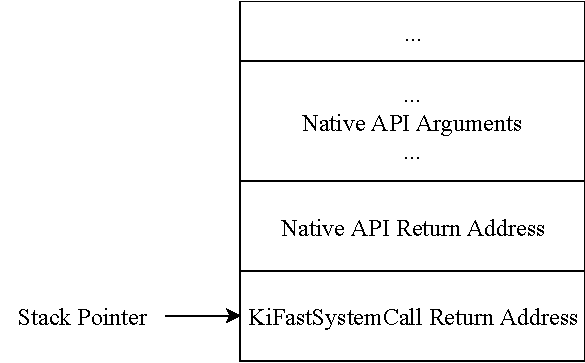
\includegraphics[width=0.7\textwidth]{Figures/StackMainImage.pdf}
\caption{\textit{Stack before} \texttt{sysenter} \textit{execution}}
\end{figure}     

Having outlined the general situation, it is finally possible to describe how the main image check is carried out:

\begin{enumerate}
\item The first check involves discovering whether or not \texttt{sysenter} is called directly from the main executable. As Pin intercepts Native APIs right before the execution of \texttt{sysenter}, this can be trivially done by checking if the instruction pointer value obtained in \texttt{TraceSysCallEntry} falls within the main executable memory address range.
\item Secondly, it is required to examine if the Native API return address belongs to the main executable. As a result of what shown in \textit{Figure 3.3} such return address is obtained by adding 4 to the stack pointer and retrieving the pointed value, where the stack pointer can be obtained in Pin through the use of \texttt{PIN\_GetContextReg}. The resulting value is then, once more, compared with the main executable memory address range.
\end{enumerate}

\subsection{Native API Name Resolution}

Previously, it was stated how it is possible to register a callback function to be executed before Native APIs through the use of \texttt{PIN\_AddSyscallEntryFunction}. Such callback functions, named \texttt{SYSCALL\_ENTRY\_CALLBACK}s, receive a set of parameters, including \texttt{ctx}, the application's register state immediately before the system call execution, and \texttt{std}, the system call standard. In Blue Pill, these two parameters are used to invoke \texttt{PIN\_GetSyscallNumber} inside its \texttt{SYSCALL\_ENTRY\_CALLBACK}. Such API returns the number (ID) of the Native API to be executed in the provided context \cite{Pin}.

Blue Pill employs a mechanism which allows it to obtain the Native API name from its number, since the hooking functions it employs are indexed by name and not by ordinal. This choice was made because the identifiers vary depending on the Windows version, even among different Service Pack versions. For the same reason, the information needed by BlueTracer to correctly log Native APIs is also indexed by Native API name and, consequently, BlueTracer also utilizes the aforementioned Native API name resolution mechanism.

The idea is to create an array, named \texttt{syscallIDs}, where Native API names are indexed by their IDs, by parsing \texttt{ntdll}'s export information. The export data of a PE is stored in the \texttt{IMAGE\_EXPORT\_DIRECTORY} structure located in the header. In our case, the most relevant fields of this structure are:

\begin{itemize}
\item The \texttt{AddressOfFunctions} array, which contains RVAs \footnote{A RVA (Relative Virtual Address) is essentially an offset within the PE image in memory} pointing to the actual exported functions and is indexed by an export ordinal.
\item The \texttt{AddressOfNames} array, which is an array of 32-bit RVAs pointing to symbol strings.
\item The \texttt{AddressOfNameOrdinals} array, which is an array of 16-bit ordinals existing in parallel with \texttt{AddressOfNames}, i.e. they possess the same number of elements and there is a direct relation between equivalent indices \cite{Sikorski:2012:PMA:2181153}.  
\end{itemize}

\newpage

With this in mind, \texttt{syscallIDs} is built by carrying out the following actions for every element \texttt{iName} in \texttt{AddressOfNames}:

\begin{enumerate}
\item The corresponding \texttt{AddressOfNameOrdinals} element is retrieved, i.e. the one with the same index. Let us call this value \texttt{iOrdinal}.
\item \texttt{iOrdinal} is used to index in \texttt{AddressOfFunctions}. This time the obtained value is the RVA pointing to the exported function.
\item The pointed function is expected to begin \texttt{mov eax, syscall\_number}. As a result of this, the first byte should be \texttt{B8h} and the syscall number can be obtained by considering the next four bytes.  
\end{enumerate}

By following the above procedure, every element in \texttt{AddressOfNames} can be therefore mapped to the corresponding identifier. 

\subsection{Native API Information Representation and Retrieval}

When tracing Native APIs, it is wanted to record as much data as possible as well as correctly formatting the arguments' values. To do this, it is required to have access to some kind of source of Native API related information, which can assist the tracer in the logging activity by, for example, providing the number of arguments a Native API takes as input, listing the arguments' types and differentiating between input and output arguments.
In BlueTracer, this information was adapted from the Native API data provided by Dr.Memory \cite{DrMemory}, a memory monitoring tool based on the DynamoRIO DBI framework.

For each Native API, the information related to it is contained in a \texttt{struct} of type \texttt{syscall\_info\_t} (\textit{Listing 3.2}). Most fields of such \texttt{struct} are self-explanatory. In particular, \texttt{num} is a \texttt{struct} storing two values indicating the system call number; these are filled in dynamically by Dr.Memory but are not needed by BlueTracer. Furthermore, the \texttt{flags} field is utilized to notify whether or not all the details of the Native API are known, as most Native APIs are undocumented. Undoubtedly though, a major role is played by the \texttt{arg} array, which is made up by \texttt{sysinfo\_arg\_t} \texttt{struct}s (\textit{Listing 3.2}) containing the data of the Native API arguments. This array is initialized with size \texttt{MAX\_ARGS\_IN\_ENTRY} (i.e. 18), since a Native API can have at most 18 arguments. 
\\
\begin{lstlisting}[caption={\texttt{struct} containing Native API-related information},captionpos=b]
	typedef struct _syscall_info_t {

		drsys_sysnum_t num;			// Native API ID
		const char *name;			// Native API Name
		uint flags; 				// SYSINFO_ flags
		uint return_type; 			// Return type
		int arg_count;				// Number of arguments

		// Array of arguments
		sysinfo_arg_t arg[MAX_ARGS_IN_ENTRY];

		...
	} syscall_info_t;
\end{lstlisting}

\begin{lstlisting}[caption={\texttt{struct} containing information associated to a Native API argument},captionpos=b]
	typedef struct _sysinfo_arg_t {
		int param; 				    // Parameter Ordinal
		int size; 				    // Size
		uint flags; 				// SYSARG_ flags
		int type; 				    // Type
		const char *type_name; 	    // Symbolic Name of the arg Type
	} sysinfo_arg_t;
\end{lstlisting}

In \texttt{sysinfo\_arg\_t}, other than \texttt{param} and \texttt{size}, that are straightforward, the following fields are also present:
\begin{itemize}
\item \texttt{flags}, which stores an \texttt{OR} of flags describing the argument's characteristics. The most important ones are:

\begin{itemize}
\item \texttt{SYSARG\_READ (R)} : input argument. 
\item \texttt{SYSARG\_WRITE (W)} : output argument.
\item \texttt{SYSARG\_INLINED} : non-memory argument, i.e the whole value is in parameter slot.
\item \texttt{SYSARG\_HAS\_TYPE (HT)} : argument with a type specifier. In fact, a non \texttt{SYSARG\_INLINED} argument is by default of type \texttt{struct} (\texttt{DRSYS\_TYPE\_STRUCT}), unless specified otherwise by \texttt{SYSARG\_HAS\_TYPE}. 
\end{itemize}

\item \texttt{type}, which is an \texttt{enum} value indicating the data type of the parameter

\item \texttt{type\_name}, a string indicating the symbolic name of the \texttt{arg} type, which is typically filled dynamically based on the \texttt{type} value. In case the argument value is a named constant, the \texttt{type\_name} field contains the name of the enumeration the constant belongs to. In fact, for each one of these enumerations, BlueTracer has access to a \texttt{struct} specific for that enumeration containing the constant values and their corresponding name. This information was also provided by Dr.Memory and is employed to translate constants to the appropriate name, as it will be explained in the next section. 

\end{itemize}

To make things clearer, an instance of \texttt{syscall\_info\_t} for the Native API \texttt{NtAllocateVirtualMemory} was provided in the listing below (\textit{Listing 3.4}).
\\
\begin{lstlisting}[caption={Instance of \texttt{syscall\_info\_t} relative to \texttt{NtAllocateVirtualMemory}},captionpos=b]
	{ { 0,0 },"NtAllocateVirtualMemory", OK, RNTST, 6,
	{
		{ 0, WIN_SIZE(HANDLE), SYSARG_INLINED, DRSYS_TYPE_HANDLE },
		{ 1, WIN_SIZE(PVOID), R | WR | HT, DRSYS_TYPE_POINTER },
		{ 2, WIN_SIZE(ULONG), SYSARG_INLINED, DRSYS_TYPE_UNSIGNED_INT },
		{ 3, WIN_SIZE(ULONG), R | WR | HT, DRSYS_TYPE_UNSIGNED_INT },
		{ 4, WIN_SIZE(ULONG), SYSARG_INLINED, DRSYS_TYPE_UNSIGNED_INT, "MEM_COMMIT" },
		{ 5, WIN_SIZE(ULONG), SYSARG_INLINED, DRSYS_TYPE_UNSIGNED_INT, "PAGE_NOACCESS" },
	}
\end{lstlisting}

In \textit{3.2.2} it was explained how BlueTracer obtains a Native API name from its ID. After that, as shown in \textit{Figure 3.2}, there must be a way to, given a specific Native API name, retrieve the corresponding \texttt{syscall\_info\_t struct}. This is done by building an hash map during the tool's initialization which maps the Native API name to the appropriate \texttt{struct}. Such idea is also adopted for named constants enumerations since a hash map is also constructed with the objective of associating the name of a named constant enumeration to the corresponding \texttt{struct}.    

\subsection{Native API Logging}
With reference to \textit{Figure 3.2}, let us consider the point in \texttt{TraceSysCallEntry} where the \texttt{syscall\_info\_t struct} relative to the Native API being traced was successfully retrieved. Before describing how the logging of "known" Native APIs is performed, it is worth mentioning that, in case a \texttt{struct} describing a certain Native API is not found, BlueTracer just logs the name of the Native API and the input value of a user-specified number of arguments (4 by default).

The first step towards logging "known" Native APIs is allocating and initializing a \texttt{syscall\_tracer struct} (\textit{Listing 3.5}) representing the specific Native API being traced. This \texttt{struct} is built starting from the data present in the previously retrieved  \texttt{syscall\_info\_t struct} and it is at the heart of the logging of the Native API.
\\
\begin{lstlisting}[caption={\texttt{struct} representing the Native API being traced},captionpos=b]
	typedef struct _syscall_tracer {
		ADDRINT syscall_number;			// Native API ID
		const char * syscall_name;		// Native API Name
		int argcount;				    // Number of Arguments

		// Array of arguments
		drsys_arg_t arguments[MAX_ARGS_IN_ENTRY];

		drsys_arg_t retval;			    // Return value
		int syscall_counter;			// Native API Counter
	} syscall_tracer;
\end{lstlisting}

Even for \texttt{syscall\_tracer}, each field is self-explanatory. The only one which was not encountered before is the \texttt{syscall\_counter} field. The rationale behind this field is that, in the log, each traced call has a unique integer associated to it, utilized to group together the information relative to the call in post-processing. The next identifier to be assigned is stored in the \texttt{call\_number} field of the thread local storage (\textit{Listing 3.1}). Therefore, \texttt{syscall\_counter} simply contains the unique identifier associated to the Native API in the log. The arguments of a specific Native API are represented via the \texttt{drsys\_arg\_t} struct (\textit{Listing 3.6}).
\\
\begin{lstlisting}[caption={\texttt{struct} representing the an argument of the Native API being traced},captionpos=b]
typedef struct _drsys_arg_t {

	// Whether operating pre-call (if true) or post-system call (if false)
	bool pre;

	int ordinal;			    // Parameter Ordinal				
	int size;			        // Size	
	uint flags;			        // SYSARG_ flags
	int type;			        // Type
	const char *type_name;		// Symbolic Name of the arg Type

	// String describing the symbolic name of a named constant's enum
	const char *enum_name;

	// Argument value
	ADDRINT value;
	
} drsys_arg_t
\end{lstlisting}

\texttt{drsys\_arg\_t}'s fields are mostly the same of \texttt{sysinfo\_arg\_t}, with three additions:
\begin{itemize}
\item \texttt{pre}, which is a boolean flag set to \texttt{true} when the logging is occurring before the Native API is executed (i.e. in \texttt{TraceSysCallEntry} and set to false when the logging is occurring after the Native API is executed (i.e. in \texttt{TraceSysCallExit}).
\item \texttt{enum\_name}, a string containing the symbolic name of the enumeration a named constant belongs to. In most cases, this is the symbolic name associated to the first constant of the enumeration. Such field was introduced to decouple type name and enumeration name.
\item \texttt{value}, an \texttt{ADDRINT}\footnote{The ADDRINT type is defined by Pin and represents a memory address} containing the value of the argument. This is obtained through the \texttt{PIN\_GetSyscallArgument} API, which takes as input the context before the execution of the system call, the system call standard and the ordinal number of the argument whose value is requested.  
\end{itemize}

As previously mentioned in section 3.1.1, each thread possesses its own log file, whose pointer resides in the thread local storage, and writes on it by means of the \texttt{file\_write} function, also located in the thread local storage (\textit{Listing 3.1}). The first Native API component being logged is its name and this is done with the following format:
\\ 
\texttt{\textasciitilde\textasciitilde[System ID of thread]\textasciitilde\textasciitilde} \texttt{ [Call Counter] [Image Name]![Native API Name]}  
In the context of Native APIs, the name of the image is always \texttt{ntdll}, but this is not the case when tracing APIs.

Argument logging is done via the \texttt{print\_arg} function (\textit{Listing 3.7}), which is structured as follows:

\begin{itemize}
\item Firstly, it is determined if the argument being logged is a named constant, i.e. it is checked if \texttt{enum\_name} is different from \texttt{NULL}. In that case, the \texttt{get\_arg\_syname} function is invoked, which is in charge of, given the input named constant value, finding the corresponding name and recording it to the log. The named constant resolution is carried out by initially fetching the \texttt{struct} containing all the members of the enumeration the named constant belongs to, through the use of the aforementioned hash map. Then, it is determined if there is a perfect match between the argument value and one of the values of the \texttt{struct}'s entries. If this occurs, then the associated symbolic name is simply retrieved from the \texttt{struct}'s entry. Otherwise, a linear search is performed to unveil possible composite named constants (e.g. \texttt{FILE\_SHARED\_READ | FILE\_SHARED\_WRITE}).    

\end{itemize}

\vspace{1em}
\begin{lstlisting}[caption={\texttt{print\_arg} function},captionpos=b]
static void print_arg(drsys_arg_t* curr_arg, bluepill_tls* tdata, uint syscall_counter) {

	...

	// Constant Resolution
	if (curr_arg->enum_name != NULL) {
		if (get_arg_symname(curr_arg, tdata))
			return;
	}

	switch (curr_arg->type) {
		case DRSYS_TYPE_VOID:	      print_simple_value(curr_arg, true, tdata); break;
		case DRSYS_TYPE_POINTER:      print_simple_value(curr_arg, true, tdata); break;
		case DRSYS_TYPE_BOOL:         print_simple_value(curr_arg, false, tdata); break;
		case DRSYS_TYPE_INT:          print_simple_value(curr_arg, false, tdata); break;
		case DRSYS_TYPE_SIGNED_INT:   print_simple_value(curr_arg, false, tdata); break;
		case DRSYS_TYPE_UNSIGNED_INT: print_simple_value(curr_arg, false, tdata); break;
		case DRSYS_TYPE_HANDLE:       print_simple_value(curr_arg, false, tdata); break;
		case DRSYS_TYPE_NTSTATUS:     print_simple_value(curr_arg, false, tdata); break;
		case DRSYS_TYPE_ATOM:         print_simple_value(curr_arg, false, tdata); break;
	default: {
		if (curr_arg->value == 0) {
			(tdata->file_write)(tdata->threadid, tdata->buffer, tdata->OutFile, "<null>");
		}
		else if (curr_arg->pre && !TEST(SYSARG_READ, curr_arg->flags)) {
			(tdata->file_write)(tdata->threadid, tdata->buffer,
			tdata->OutFile, PFX, curr_arg->value);
		}
		else {
			if (!print_known_compound_type(curr_arg, tdata))
				(tdata->file_write)(tdata->threadid, tdata->buffer, tdata->OutFile, "<NYI>");
		}
	}
	...
}
\end{lstlisting}

\begin{itemize}
\item Then, if the argument's type is primitive (e.g. \texttt{int}, \texttt{bool}, etc.),  \texttt{print\_simple\_value} is invoked to record its value. In particular the second parameter of this function is a boolean which is set to \texttt{true} if it is wanted to print the argument's value with leading zeros (e.g. if the argument is of pointer type and the address it stores is being logged ) and \texttt{false} otherwise. The way \texttt{print\_simple\_value} operates is quite straightforward:
\begin{enumerate}
\item At the beginning the argument's value is simply logged, with leading zeroes or not depending on the previously mentioned parameter
\item Then, if the argument is a pointer, it is determined if the value it points to needs to be logged. This occurs if the argument is being processed before the Native API execution (i.e. \texttt{pre} is \texttt{true}) and is an input parameter (i.e. SYSARG\_READ is contained in \texttt{flags}) or if the argument is being processed after the Native API execution (i.e. \texttt{pre} is \texttt{false}) and is an output parameter (i.e. SYSARG\_WRITE is contained in \texttt{flags}). The pointed value is obtained through the use of \texttt{PIN\_SafeCopy}, which copies the specified number of bytes from a source memory region to a destination memory region, guaranteeing safe return to the caller even if such regions are inaccessible.  
\end{enumerate}      

\item Finally, if the argument's type is not a primitive one, it is checked if it is \texttt{null} and if it is a complex output parameter being traced before the Native API execution, situation in which only the address stored in the pointer is logged. If none of these two scenarios are true, then the tracer finds itself in the situation where it is required to log the value of a complex type. This is performed through the invocation of \texttt{print\_known\_compound}. As of right now, such function differentiates between four complex types, namely \texttt{UNICODE\_STRING}, \texttt{OBJECT\_ATTRIBUTES}, \texttt{IO\_STATUS\_BLOCK} and \texttt{LARGE\_INTEGER}, and logs the argument's value accordingly. If the argument's type is a complex type that is not supported, the symbolic value \texttt{<NYI>} (not yet implemented) is recorded.    

\end{itemize}

Once the arguments' input values are logged, then the reference to the \texttt{syscall\_tracer struct} representing the Native API under analysis is stored in thread local data (\textit{Listing 3.1}). This is done so that, after the Native API's execution, the corresponding \texttt{syscall\_tracer} data structure can be accessed from \texttt{TraceSysCallExit}. In fact, as mentioned in section 3.2, the \texttt{bluepill\_tls struct} associated to the running thread can be retrieved in any analysis function by means of \texttt{PIN\_GetThreadData}.

In \texttt{TraceSysCallExit}, after the value of \texttt{syscallEntry} has been fetched from the thread local storage, then it is determined whether the Native API has succeeded by checking if the output of \texttt{PIN\_GetSyscallErrno} is equal to zero, where \texttt{PIN\_GetSyscallErrno} is a Pin API returning the error code of the system call which has just returned with the provided context. Afterwards, \texttt{PIN\_GetSyscallReturn} is utilized to get the return value of the Native API and, with this information, the corresponding \texttt{drsys\_arg\_t} data structure is built. Successively, the Native API return value is logged, together with the output arguments, using once again \texttt{print\_arg} (\textit{Listing 3.7}). Finally, the \texttt{syscall\_tracer struct} representing the Native API being traced is deallocated.

To conclude this section, let us show how a traced Native API looks like in the log file (\textit{Figure 3.4}). As it can be observed, the adopted log format is quite intuitive. In fact, the idea was to have a log which is both easy to read by the analyst but also easy to parse and post-process.      
\\

\lstset{
    language=C++,
    frame=tb, % draw a frame at the top and bottom of the code block
    tabsize=4, % tab space width
    showstringspaces=false, % don't mark spaces in strings
    numbers=none, % display line numbers on the left
    commentstyle=\color{ao}, % comment color
    keywordstyle=\color{blue}, % keyword color
    stringstyle=\color{red}, % string color
    basicstyle=\footnotesize\ttfamily,
    basewidth = {.48em}
}
\begin{lstlisting}[caption={Log entry relative to a \texttt{NtOpenFile} call},captionpos=b]
~~2868~~ 1072 ntdll.dll!NtOpenFile
1072 	arg 0: 0x000fe810 (type=HANDLE*, size=0x4)
1072 	arg 1: 0x100020 (type=unsigned int, size=0x4)
1072 	arg 2: len=0x18, root=0x0, name=210/538 "\??\C:\Windows\WinSxS\
		x86_microsoft.windows.gdiplus_6595b64144ccf1df_1.1.7601.23894_none_5c0be957a009922e", 
		att=0x40, sd=0x00000000, sqos=0x00000000 (type=OBJECT_ATTRIBUTES*, size=0x4)
1072 	arg 3: 0x000fe7c0 (type=IO_STATUS_BLOCK*, size=0x4)
1072 	arg 4: FILE_SHARE_READ|FILE_SHARE_WRITE (type=named constant, value=0x3, size=0x4)
1072 	arg 5: FILE_DIRECTORY_FILE|FILE_SYNCHRONOUS_IO_NONALERT
 		(type=named constant, value=0x21, size=0x4)
1072    succeeded =>
1072 	arg 0: 0x000fe810 => 0x58 (type=HANDLE*, size=0x4)
1072 	arg 3: status=0x0, info=0x1 (type=IO_STATUS_BLOCK*, size=0x4)
\end{lstlisting}
\lstset{
    language=C++,
    frame=tb, % draw a frame at the top and bottom of the code block
    tabsize=4, % tab space width
    showstringspaces=false, % don't mark spaces in strings
    numbers=left, % display line numbers on the left
    commentstyle=\color{ao}, % comment color
    keywordstyle=\color{blue}, % keyword color
    stringstyle=\color{red}, % string color
    basicstyle=\footnotesize\ttfamily,
    basewidth = {.48em}
}

\section{APIs Tracing}

In Microsoft Windows, APIs are implemented as functions provided by a set of dynamic-link libraries. These, also known as DLLs, constitute Microsoft's way of implementing the concept of shared libraries in the Windows operating system. Therefore, the functions they make available can be employed by different applications \cite{DLL}. Windows APIs offer a plethora of functionalities which belong to many different categories, ranging from base services (e.g. file management) to user interface functions and network operations \cite{WinAPI}. In light of this, a Windows API has rich semantic information associated to it and tracing the sequence of APIs a malware calls provides analysts with a very high-level view of the sample's behavior. This is why BlueTracer's API tracer component is undoubtedly the most important one. 
\\
\begin{figure}[h]
\centering
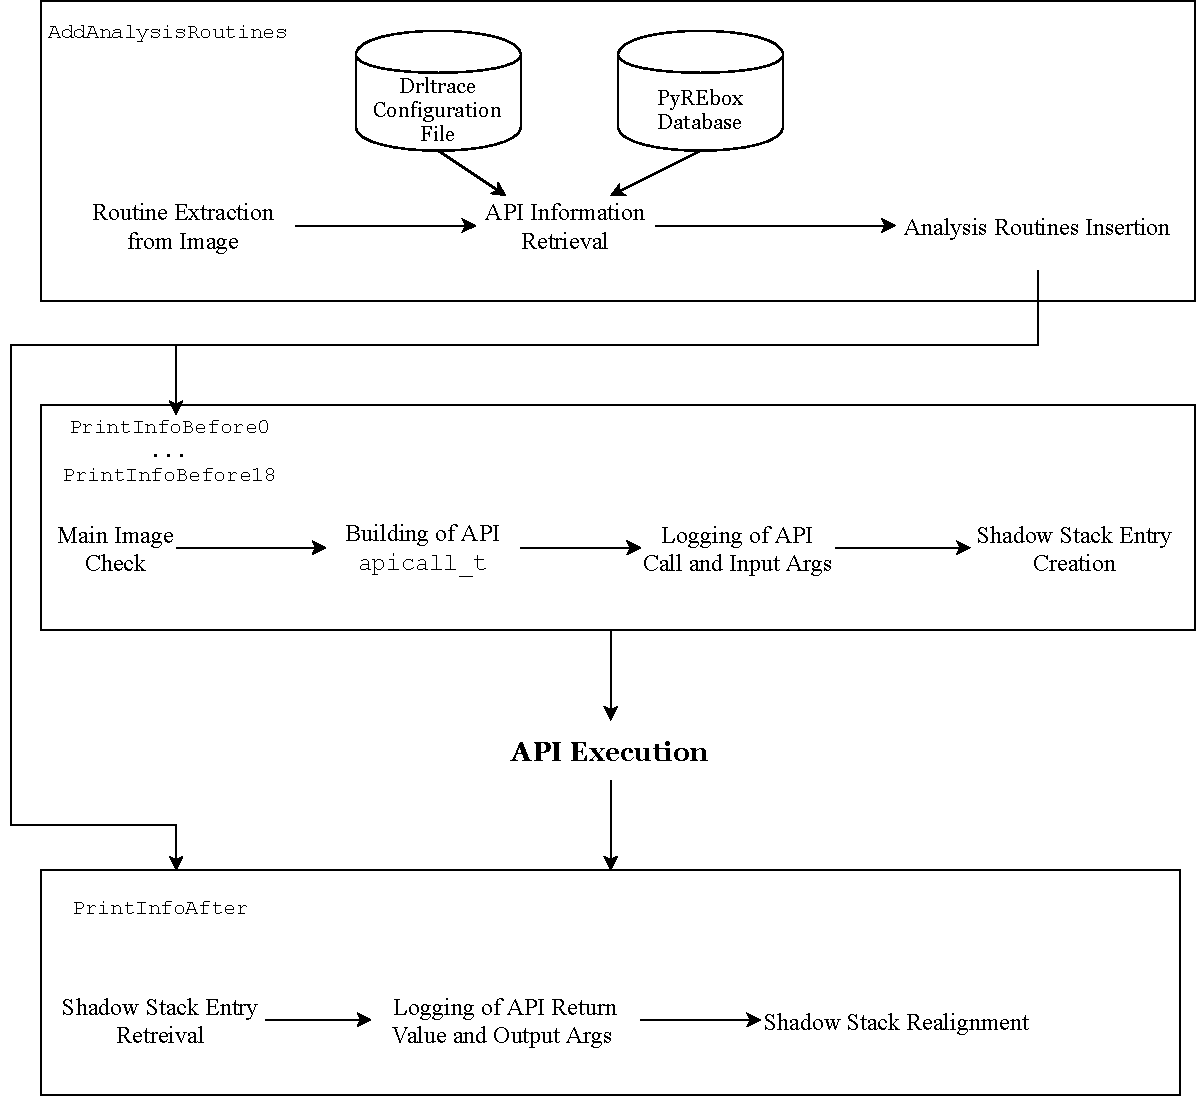
\includegraphics[scale=0.662]{Figures/APITracing.pdf}
\caption{\textit{APIs Tracing Workflow}}
\end{figure}

 
When tracing APIs, most of the concepts seen in Native API tracing also apply, but there are also significant differences, both in the steps that were carried out and in the Pin APIs which were employed, as it can be observed from the diagram in \textit{Figure 3.4}.

Now let us illustrate the actions being performed during API tracing by analyzing in detail each one of the three main blocks of \textit{Figure 3.4}.

\subsection{APIs Instrumentation}

The first step taken towards APIs tracing is APIs instrumentation, i.e. placing analysis routines before and after the APIs' execution. To do this, a specific function was embedded in Blue Pill's image callback (the notion of image callback was previously introduced in Section 3.3.1). Such function, named \texttt{AddAnalysisRoutines}, performs the following actions for every DLL being loaded:

\begin{enumerate} 
\item It inspects the symbol table, i.e. the DLL's exports. To this end, Pin symbol objects (\texttt{SYM}s) are employed, which provide information about function symbols in the applications \cite{Pin}.
\item For every symbol object, it retrieves the corresponding routine (\texttt{RTN}) object. In fact, in Pin a \texttt{RTN} represents a function usually generated by a compiler for a procedural programming language, e.g C \cite{Pin}. To retrieve the aforementioned \texttt{RTN} object, the \texttt{RTN\_FindByAddress} API was utilized, which takes as input a \texttt{RTN} memory address and returns an handle to the found \texttt{RTN}. Such memory address was determined by adding the symbol's RVA (obtained via \texttt{SYM\_Value}) to the lowest image address (fetched through \texttt{IMG\_LowAddress}).  
\item For every routine object, it retrieves the corresponding name via \texttt{RTN\_name} and checks whether or not the API being represented is "known", i.e. a source of information associated to the API exists.

\begin{itemize}
\item If the API is not "known", it adds an analysis routine just before the API's execution, which simply logs the value of a user-specified number of args (four by default), exactly like what happens in NTAPIs tracing.
\item If the API is "known", it adds analysis routines before and after the API's execution, which log detailed information relative to the API, including the arguments' input and output values. 
\end{itemize}
 
\end{enumerate}

Having given a general outline on how \texttt{AddAnalysisRoutine} works, let us now describe its underlying details.

Similarly to what occurs for NTAPI tracing, in order to log as much information as possible and to correctly record the arguments' values, it is necessary to have a source of API information, providing some kind of assistance during the tracing activity. When dealing with APIs, BlueTracer allows the user to choose between two possible sources of API information: \textit{drltrace}'s configuration file or the data extracted from \textit{PyREbox}'s database. By default, the latter is employed as it embodies a greater amount of information, including variable names and named constants' enumerations.

\textit{drltrace} (already mentioned in section 2.3) comes with its own external configuration file, in which each line contains information relative to an API, as it can be observed from the sample configuration file entry below (\textit{Listing 3.9}).      
\\
\lstset{
    language=C++,
    frame=single, % draw a frame at the top and bottom of the code block
    tabsize=4, % tab space width
    showstringspaces=false, % don't mark spaces in strings
    numbers=none, % display line numbers on the left
    commentstyle=\color{ao}, % comment color
    keywordstyle=\color{blue}, % keyword color
    stringstyle=\color{red}, % string color
    basicstyle=\footnotesize\ttfamily,
    basewidth = {.48em}
}
\begin{lstlisting}[caption={Sample entry in \textit{drltrace} configuration file},captionpos=b]
bool|GetUILanguageInfo|DWORD|wchar*|__out wchar*|__inout DWORD*|__out DWORD*
\end{lstlisting}
\lstset{
    language=C++,
    frame=tb, % draw a frame at the top and bottom of the code block
    tabsize=4, % tab space width
    showstringspaces=false, % don't mark spaces in strings
    numbers=left, % display line numbers on the left
    commentstyle=\color{ao}, % comment color
    keywordstyle=\color{blue}, % keyword color
    stringstyle=\color{red}, % string color
    basicstyle=\footnotesize\ttfamily,
    basewidth = {.48em}
}

Each piece of information in an entry is separated by \texttt{|}. The first bit of data is the API's return type, the second is the API's name and the rest of the entry is made up by the arguments' types. In particular, the \texttt{\_\_out} token is used to mark output arguments, while \texttt{\_\_inout} is utilized to identify input and output arguments. In case there is no token, it means that the argument is just an input one. 

Before API instrumentation takes place, BlueTracer parses the aforementioned configuration file and, for every entry, builds a \texttt{sysinfo\_arg\_t struct} (\textit{Listing 3.2}) for each argument in the entry. It was decided to reuse \texttt{sysinfo\_arg\_t struct} since its fields were fitting with respect to the arguments' information which had to be stored. Therefore, after this parsing process, each configuration file entry is represented by an <API name, \texttt{vector} of \texttt{sysinfo\_arg\_t}s> pair. Such pairs are then utilized to build an hash map, which maps the API name to the corresponding arguments. This hash map is used in step 3 of the APIs instrumentation process to, given the API name, fetch the appropriate information. In particular, it is important to note that, from a performance point of view, it is much better to include the information retrieval operations in the image instrumentation function, rather than in the analysis ones, as the former are executed just once for every image, while the latter are invoked each time an API is called by the pinned application.

The other source of API information employed by BlueTracer is \textit{PyREbox}'s database. \textit{PyREbox} is a Python scriptable reverse engineering sandbox based on QEMU and VMI techniques, the goal of which is to provide support for reverse engineering through its dynamic analysis capabilities \cite{Pyrebox}. \textit{PyREbox} is equipped with its own API tracer, which relies on the information contained in a sqlite database to correctly log the APIs' parameters. Such database was, in turn, generated by utilizing as its core the data from the \textit{Deviare}\footnote{Deviare is an open-source hooking engine for instrumenting arbitrary \texttt{Win32} functions \cite{Deviare}} project and then employing a crawler for parsing the Microsoft online documentation with the goal of marking which parameters are input parameters and which are output parameters. The resulting database is incredibly richer in API information than \textit{drltrace}'s configuration file. In fact, the number of APIs for which data is stored is much higher, argument names are also included, as well as the contents of named constants' enumerations, information which \textit{drltrace}'s configuration file does not provide at all.

In order to extract information relative to the APIs from PyREbox's database, a Python script was employed, which, for every API, instantiates a \texttt{libcall\_info\_t struct} (\textit{Listing 3.10}) in a \texttt{.cpp} file.
\\
\begin{lstlisting}[caption={\texttt{struct} containing API-related information from PyREbox's database},captionpos=b]
typedef struct _libcall_info_t {
	const char* func_name;     			// API name
	int argnum;				   			// Number of Args
	libcall_arg_info_t lib_args[19];	// Array of arguments
} libcall_info_t
\end{lstlisting}
\vspace{1cm}

The most important field of such \texttt{struct} is surely the arguments' array, which is made up of \texttt{libcall\_arg\_info\_t} data structures (\textit{Listing 3.11}) containing the information relative each argument of an API, including an entry specific for the return value data. The array size was set to 19, since it was observed from the database data that the API with the most parameters had 18 arguments. This time, it was decided not to reuse NTAPI's \texttt{sysinfo\_arg\_t struct} (\textit{Listing 3.2}) to store the API's arguments information due to its lack of the field storing the argument name. 
\\
\begin{lstlisting}[caption={\texttt{struct} containing information associated to an API argument},captionpos=b]
typedef struct _libcall_arg_info_t {

	int arg_num;				// Arg Ordinal
	const char* arg_name;		// Arg Name
	int arg_type;             	// Arg Type
	char* arg_type_name;		// Arg Type Name
	int size;					// Size
	bool in_out_flag;			// Input/Output Flag

} libcall_arg_info_t;
\end{lstlisting}   

Although \texttt{libcall\_arg\_info\_t}'s fields seem to be pretty self-explanatory, let us quickly go through them to reveal some details which are not so obvious:

\begin{itemize}
\item \texttt{arg\_num} is an \texttt{int} which contains the argument's ordinal. In case the return value is being represented, it is set to -1.
\item \texttt{arg\_name} is a string containing the argument name as reported by Microsoft's official documentation.
\item \texttt{arg\_type} is an \texttt{int} from an enumeration representing the argument's type. In particular, differently from the strategy adopted from Native APIs, in case of a pointer the \texttt{NKT\_DBOBJCLASS\_Pointer} enumeration member is ORed with an \texttt{int} representing the pointed type. The same thing happens in case of a pointer to a pointer but with the \texttt{NKT\_DBOBJCLASS\_PointerPointer} flag being used instead. This was done to reflect how API information is stored inside the database.
\item \texttt{arg\_type\_name} is a string which is used in the three specific scenarios below, according the type of the argument, and is \texttt{null} otherwise:
\begin{enumerate}
\item To store the symbolic name of an enumeration.
\item To store the \texttt{struct} type name.
\item To store the \texttt{union} type name.
\end{enumerate}
\item \texttt{size} is an \texttt{int} storing the argument's size. In case of a pointer (or a pointer to a pointer) the size of the pointed type is stored.
\item \texttt{in\_out\_flag} is a \texttt{bool} which is set to \texttt{INOUT} (i.e \texttt{true}) if the represented argument is an output argument and \texttt{IN} (i.e. \texttt{false}) otherwise. This means that, by default, all the arguments are considered as input arguments and are therefore traced before the API execution, while only the arguments for which \texttt{in\_out\_flag} is \texttt{true} are traced after the API's execution.
\end{itemize}

To give a better idea on how API data is represented, an instance of \texttt{libcall\_arg\_info\_t} containing the information associated to \texttt{WriteFileEx} can be observed below (\textit{Listing 3.12}).
\\
\begin{lstlisting}[caption={Instance of \texttt{libcall\_arg\_info\_t} relative to \texttt{WriteFileEx}},captionpos=b]
	{ "WriteFileEx",5,
	{ 
		{-1, "Return value", NKT_DBFUNDTYPE_SignedDoubleWord, 0, 4, INOUT },
		{0, "hFile", NKT_DBFUNDTYPE_UnsignedDoubleWord, 0, 4, IN },
		{1, "lpBuffer", NKT_DBFUNDTYPE_Void | NKT_DBOBJCLASS_Pointer, 0, 0, IN },
		{2, "nNumberOfBytesToWrite", NKT_DBFUNDTYPE_UnsignedDoubleWord, 0, 4, IN },
		{3, "lpOverlapped", NKT_DBOBJCLASS_Struct | NKT_DBOBJCLASS_Pointer,
		 "_OVERLAPPED", 160, INOUT },
		{4, "lpCompletionRoutine", NKT_DBOBJCLASS_Typedef, 0, 0, IN },
	}
	}
\end{lstlisting}

Due to the high amount of APIs for which information was stored in the \texttt{PyREbox} database, it was decided to group API data by DLL. Specifically, for every DLL a corresponding \texttt{.cpp} file was created to store the API-related information under the form of \texttt{libcall\_arg\_info\_t} instances, one for each "known" API exported by that DLL. Furthermore, in order to make API data retrieval more efficient, it was chosen to employ a two-level hash map approach for this purpose. Given the DLL name (easily obtainable in the image callback via the use of \texttt{IMG\_Name}), the first level hash map is utilized to retrieve the DLL-specific second level hash map, which, in turn, maps the API name to the appropriate \texttt{struct} instance (\textit{Figure 3.5}). This is how API information retrieval is carried out in case \textit{PyREbox} database is used as API data source.
\\
\begin{figure}[h]
\centering
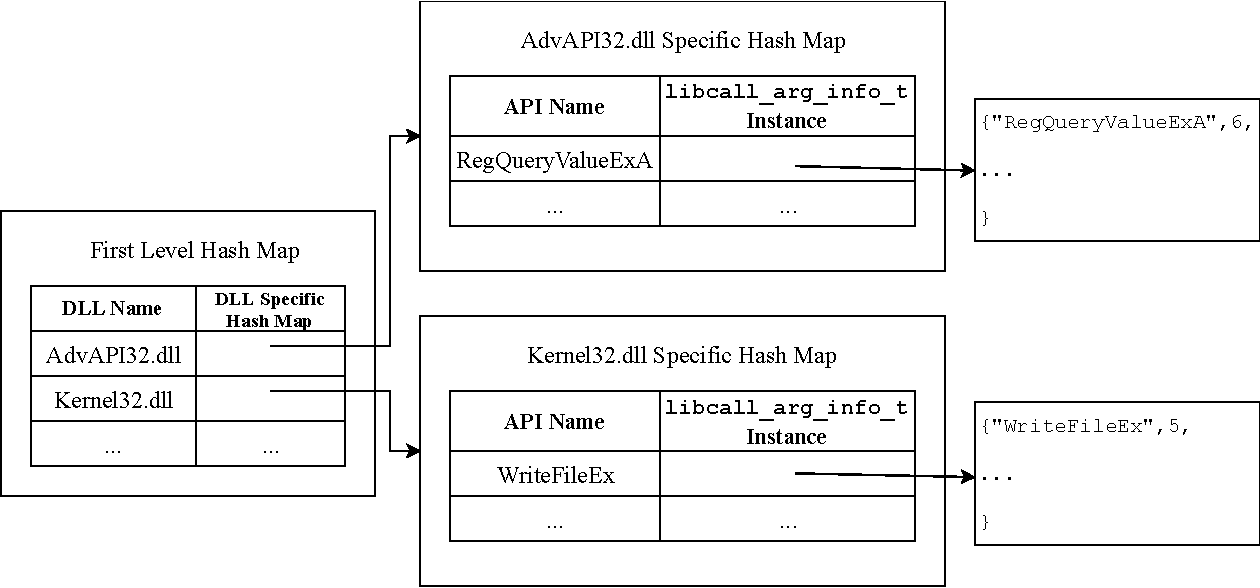
\includegraphics[width=1\textwidth]{Figures/HashMap.pdf}
\caption{\textit{PyREbox API Information Retrieval}}
\end{figure}

Let us conclude this section by explaining how analysis routines are inserted before and after the API execution during the API instrumentation procedure outlined in page 31. In BlueTracer such operation heavily relies on the use of the \texttt{RTN\_InsertCall}, which allows to insert analysis functions relative to a \texttt{RTN} object. This API takes as input the following parameters:
\begin{itemize}
\item The routine object (\texttt{RTN}) representing the function under analysis.
\item A member of the \texttt{IPOINT} enumeration which determines where the analysis function is inserted in relation to the instrumented object. It can be either \texttt{IPOINT\_BEFORE}, in which case the analysis code is placed before the instrumented function, or \texttt{IPOINT\_AFTER}, in which case the analysis code is placed after the instrumented function.
\item The analysis function to be called.
\item The arguments to pass to the analysis function, specified via members of the \texttt{IARG\_TYPE} enumeration. If the analysis function is placed before the instrumented object, then such arguments may also include the parameters' values of the function being instrumented. However, for this to occur the pair <\texttt{IARG\_FUNCARG\_ENTRYPOINT\_VALUE}, argument number> needs to be included for each of the analyzed function's parameters. Conversely, to obtain the instrumented function's result, \texttt{IARG\_FUNCRET\_EXITPOINT\_VALUE} is required. Obviously, this is possible only if the analysis function is placed after the instrumented object.
\end{itemize}

In BlueTracer, the number of arguments of the API being traced is known only after the API-related information has been retrieved. Because of this and given Pin's way of passing the arguments to the analysis functions, a \texttt{switch} had to be employed when adding analysis functions before the API execution. Such \texttt{switch}, given the API arguments' number, places the appropriate analysis function, i.e. the one with the number of <\texttt{IARG\_FUNCARG\_ENTRYPOINT\_VALUE}, argument number> pairs equal to the number of arguments the API takes. This is done in order to ensure that the analysis function receives all the values of the API's arguments before the API's execution. As a result, in BlueTracer there are 19 (one for zero arguments as well) different API \texttt{IPOINT\_BEFORE} analysis functions, named \texttt{PrintInfoBefore[Arguments' Number]}, which vary only in the number of APIs' argument values they receive in input. Obviously this is true just for "known" APIs. In case the API under analysis is not "known", then the number of API argument values is always the same and the \texttt{switch} is not required.

Let us now dissect an invocation of \texttt{RTN\_InsertCall} to further clarify how BlueTracer adds analysis code before the execution of an API (\textit{Listing 3.13}).  
\begin{lstlisting}[caption={\texttt{RTN\_InsertCall} invocation to add analysis code before an API's execution},captionpos=b]
RTN_InsertCall(rtn, IPOINT_BEFORE, (AFUNPTR)PrintInfoBefore[Number of API Args],
 	IARG_FAST_ANALYSIS_CALL,
	IARG_ADDRINT, argNumber,
	IARG_ADDRINT, libPointer, IARG_ADDRINT, rtn_name, IARG_ADDRINT, img_name,
	IARG_REG_VALUE, REG_STACK_PTR,
	IARG_THREAD_ID,
	IARG_RETURN_IP,
	[Number of API Args]_ARGS
	IARG_END);
\end{lstlisting}

In particular, the arguments which are passed to the analysis routine are:
\begin{itemize}
\item \texttt{IARG\_FAST\_ANALYSIS\_CALL}. This is not a real argument but rather a way to enable faster linkage for calls to analysis functions with the objective of improving performance \cite{Pin}.
\item \texttt{argNumber}, a constant value containing the number of the analyzed API's arguments.
\item \texttt{libPointer}, a reference to the previously retrieved data structure containing API-related data.
\item \texttt{rtn\_name}, the API name.
\item \texttt{img\_name}, the DLL name.
\item The stack pointer value before the API's execution, given by the \texttt{<IARG\_REG\_VALUE, REG\_STACK\_PTR>} pair. This is necessary for the shadow stack management, which will be detailed in the next section.
\item The thread ID assigned by Pin for the calling thread, passed via \texttt{IARG\_THREAD\_ID}. This is necessary in order to access the thread local storage from the analysis function.
\item The API return address, provided by \texttt{IARG\_RETURN\_IP}. This is employed in the main image check, similarly to what explained in Section 3.3.1.
\item The API argument values. In order to make the code more readable a macro was used in this case.
\end{itemize}

For what concerns the addition of analysis code after the API's execution, the aforementioned \texttt{switch} is not necessary since \texttt{IARG\_FUNCRET\_EXITPOINT\_VALUE} is valid only at the entry point of an analysis routine and, therefore, no API argument value is passed at this stage. The analysis function which is placed after the API's execution, named \texttt{PrintInfoAfter} essentially receives the same parameters as the ones from \textit{Listing 3.13}, with the major difference that the API's return value is passed via \texttt{IARG\_FUNCARG\_EXITPOINT\_VALUE} instead of the API arguments' values.

\subsection{API Analysis before Execution}

In this section we will describe how APIs are analyzed before execution, i.e. the main steps that are carried out in the \texttt{PrintInfoBefore} functions, an overview of which is given in \textit{Figure 3.4}.
The workflow in this case is mostly the same as the one for NTAPIs' analysis, with one major difference, that is the introduction of a shadow stack used to store API entries in the thread local storage, which will be motivated later in the section.

The first thing which is done is determining whether or not the API under analysis has been invoked directly from the main executable of the Pin application. The concepts involved here are essentially the ones applying to the main image check done for Native APIs, which was detailed in \textit{Section 3.3.1}. In short, it is checked if the API's return address, which is passed to the analysis function through the use of \texttt{IARG\_RETURN\_IP}, falls into the main executable memory address range, which was previously determined via \texttt{IMG\_HighAddress} and \texttt{IMG\_LowAddress}.

Afterwards, similarly to what occurs when logging "known" Native APIs, a \texttt{apicall\_t struct} (\textit{Listing 3.14}) representing the specific API being traced is allocated and initialized. The fields of such \texttt{struct} are all trivial and, as what done for Native API tracing, the API arguments are represented via a \texttt{drsys\_arg\_t} (\textit{Listing 3.6}) array with size \texttt{MAX\_ARGS\_CONFIG} (i.e. 18) as this is the maximum number of observed arguments for any "known" API. In particular, the \texttt{drsys\_arg\_t struct} could be reused in the context of APIs since, unlike \texttt{sysinfo\_arg\_t}, its fields could hold all API arguments' data, both from the \textit{drltrace} configuration file and the \textit{PyREBox} database, including the argument name. 
\\
\begin{lstlisting}[caption={\texttt{struct} representing the API being traced},captionpos=b]
typedef struct _apicall_t {;

	const char* img_name;							// DLL Name
	const char* rtn_name;							// API Name

	drsys_arg_t arguments[MAX_ARGS_CONFIG];			// Array of Arguments
	drsys_arg_t retval;								// Return Value
	int count;										// Arg Count

} apicall_t;
\end{lstlisting}

The \texttt{apicall\_t struct} is initialized utilizing the API-related data, which was fetched beforehand during instrumentation and was passed to the analysis function via \texttt{libPointer}, as well as the values of the API arguments, which were provided to the analysis function through \texttt{IARG\_FUNCARG\_ENTRYPOINT\_VALUE} as already discussed in \textit{Section 3.4.1}.

Then, the logging of the API proceeds exactly the same as for Native APIs: the API call is recorded employing an identical log format in order to maintain uniformity and the input values of the arguments are logged through the use of a \texttt{print\_arg} function operating exactly in the same way as the one in \textit{Listing 3.7}.

As previously hinted at, the major element which distinguishes API tracing from Native API tracing is that the former employs a shadow stack to store in the thread local storage references to the data structures representing the APIs being traced. Let us explain in detail the motivation behind such choice. It is typical for an API to call another API during its execution, forming a sort of nesting. For this reason, just storing in the thread locale storage the reference relative to the next API to be executed is not enough as this would lead to the analysis of just the most "inner" API, completely ignoring the "outer" APIs which invoked the "inner" one. Therefore, it is necessary to store not just the reference corresponding to the next API in line to be executed but rather all the references relative to the APIs for which execution has started and not yet finished. A fitting data structure to solve this issue is a shadow stack, where, for each API, the corresponding data structure is placed on top of the stack before its execution and popped from the stack after its execution has terminated, allowing both "inner" and "outer" APIs to be traced. This is why each thread has access to its own shadow stack via the \texttt{shadowStack} field in the thread local data (\textit{Listing 3.1}).

Therefore, in light of what just stated, the last operations which are done when tracing an API before its execution are allocating a shadow stack entry (\textit{Listing 3.15}), initializing it and placing it on top of the shadow stack in the thread local data, so that it can be retrieved after the API's execution.
\\
\begin{lstlisting}[caption={\texttt{struct} representing a shadow stack entry},captionpos=b]
typedef struct _stackEntry {
	apicall_t* apiInfo;    // API Call Reference
	ADDRINT  currentSP;    // Stack Pointer Register Content
	THREADID threadID;     // Thread ID
	uint api_counter;	   // Call Counter
} stackEntry;
\end{lstlisting}       

\texttt{stackEntry}'s fields are all, once again, self-explanatory. A big role in the shadow stack management is taken by the \texttt{currentSP} field, as it will be explained in the next section. Such field stores the stack pointer's value before the API's execution, which was passed to the analysis function with the <\texttt{IARG\_REG\_VALUE}, \texttt{REG\_STACK\_PTR}> pair.

\subsection{API Analysis after Execution}

Lastly, let us detail the most important operations performed towards tracing API-related information after the API execution. These are carried out in the \texttt{PrintInfoAfter} function and can be observed from \textit{Figure 3.4}.

At the beginning of \texttt{PrintInfoAfter}, the first thing which needs to be done in order to proceed with the logging is the retrieval from the shadow stack of the stack entry representing the API under analysis. A reference to the shadow stack can be easily acquired by gaining access to the thread local storage via \texttt{PIN\_GetThreadData}. However, it is not enough to pop the top of the shadow stack to obtain the wanted stack entry. This is due to a limitation of Pin in the instrumentation of routine objects.

In fact, the addition of analysis routines after a function's execution with \texttt{IPOINT\_AFTER} is implemented by instrumenting each return instruction. This does not guarantee the success of the instrumentation, meaning that, for some routines, the associated \texttt{IPOINT\_AFTER} analysis function is not executed. Therefore, in our case, it is possible that the stack entry on top of the shadow stack refers to API for which \texttt{PrintInfoAfter} has not been invoked and, therefore, the corresponding stack entry has not been popped.

As a result of this, the correct stack entry has to be fetched by iterating through the shadow stack, looking for the entry for which the values of a set of fields coincide with the values of the corresponding parameters being passed as arguments to the analysis function. Such fields are:
\begin{itemize}
\item The DLL name.
\item The API name.
\item The stack pointer value. In fact, for a given API, the stack pointer value before its execution has to be equal to the stack pointer value after its execution.
\end{itemize} 

Once the appropriate shadow stack entry has been retrieved, the API return value, which is passed to the analysis function via \texttt{IARG\_FUNCARG\_EXITPOINT\_VALUE}, is set in the \texttt{apicall\_t struct} so that it can be logged, together with the output arguments, once again utilizing the ideas behind \texttt{print\_arg} (\textit{Listing 3.7}). 

The last operation carried out by \texttt{PrintInfoAfter}, after the API under analysis has been traced, is the re-alignment of the shadow stack, i.e. the deallocation of all the stack entries belonging to APIs which have terminated their execution. In fact, due to the previously mentioned issue involving Pin's instrumentation of routines, it is necessary to manually remove from the shadow stack all the entries relative to the APIs for which the corresponding \texttt{IPOINT\_AFTER} analysis function is not executed. Such shadow stack re-alignment procedure works as follows:

\begin{enumerate}
\item The previously fetched shadow stack entry is removed.
\item All the shadow stack entries on top of the previously retrieved entry are removed. Due to their position in the stack, these entries are relative to APIs which have been called after the traced API. Such APIs, given the fact that the traced API has terminated its execution, have also finished to execute, but their relative entries have not been deallocated accordingly due to Pin's issue with routine instrumentation.
\item All the entries with a lower stack pointer value than the stack pointer value stored in the retrieved entry are removed. In fact, such entries refer, once again, to APIs which have been invoked before the traced APIs but their corresponding entries have not been deallocated accordingly.   
\end{enumerate}

\iffalse
- Shadow Stack Realignment
-> Remove all entries BEFORE in the stack
-> Remove all entries with a lower stack pointer
\fi

\section{Context Change Analysis} 

Pin has to intercept the delivery of asynchronous events from the kernel in order to keep control of the application.  
Microsoft Windows employs two mechanisms aimed at dispatching asynchronous events to user mode, i.e. callbacks and asynchronous procedure calls (APCs), both of which lead to a context change in the application \cite{5452079}.
 
In order to have a complete picture of the malware sample's activity, it is clearly relevant to also log the occurrences of such asynchronous events and to record as much information as possible related to them. Luckily, Pin provides an API which perfectly meets these needs, named \texttt{PIN\_AddContextChangeFunction}.
 
This API allows to register a notification function to execute just before the pinned application changes context due to the reception of an asynchronous event, like for instance a callback or a Windows APC. In BlueTracer, the idea is to use such registered notification function to extract and log information relative to the context change. The notification function in question is of type \texttt{CONTEXT\_CHANGE\_CALLBACK} and the most important arguments it takes as input are:
\begin{itemize}
\item A member of the \texttt{CONTEXT\_CHANGE\_REASON} enumeration indicating the reason for the context change. This is the parameter allowing BlueTracer to distinguish between callbacks and APCs. In fact, in the case of callbacks it is set to \texttt{CONTEXT\_CHANGE\_REASON\_CALLBACK}, while in the case of APCs it is set to \texttt{CONTEXT\_CHANGE\_REASON\_APC}. 
\item The application's register state before the context change. It is \texttt{null} if the context change is caused by a callback.
\item The application's register state after the context change.  
\end{itemize}      

Having outlined the tools made available by Pin to deal with the application's context changes, let us now explain in detail how callbacks tracing and Windows APCs tracing is carried out in BlueTracer.

\subsection{Callbacks Tracing}

The Windows kernel frequently needs to make callbacks in user mode with the goal of carrying out specific tasks, such as the invocation of hooks defined by the application, the provision of event notifications and the exchange of data with user mode. These calls are commonly referred to as user mode callbacks \cite{UMCallbacks}. 

To make calls from user mode to kernel mode, the user mode callback dispatcher (\texttt{KiUserCallbackDispatcher}) is employed. This function takes two arguments, a number indicating the callback to be invoked and a structure pointer which the callback receives as input, containing several parameters packed in a contiguous memory block \cite{UCDispatcher}. \texttt{KiUserCallbackDispatcher} operates in the following way:

\begin{enumerate}
\item It accesses the \texttt{KernelCallbackTable} in the process environment block \\ (PEB) \footnote{The process environment block (PEB) is a data structure employed in Windows operating systems to represent a user mode process \cite{KCT}}. The \texttt{KernelCallbackTable} is an array of function pointers, where each entry contains a reference to a callback routine \cite{KCT}.
\item It uses the callback number to locate the right routine in the array and invokes it, providing it with the aforementioned input data structure.   
\end{enumerate}

In case of a user mode callback, in Pin the registered \texttt{CONTEXT\_CALLBACK\_NOTIFICATION} function is invoked right before \texttt{KiUserCallbackDispatcher}'s execution, obviously with the reason paramater set to \texttt{CONTEXT\_CHANGE\_REASON\_CALLBACK}. 

In light of what just stated, it is natural for BlueTracer's logging activity, taking place in the registered \texttt{CONTEXT\_CALLBACK\_NOTIFICATION} function, to involve the record of a callback occurrence, together with the name of the callback that is about to be invoked. Unfortunately, tracing the callback's arguments would require further work since they are packed in a data structure, as previously explained.

Right before the execution of \texttt{KiUserCallbackDispatcher}, i.e. when the registered \texttt{CONTEXT\_CALLBACK\_NOTIFICATION} function is called, the stack looks as follows (\textit{Figure 3.6}).
\\
\begin{figure}[h]
\centering
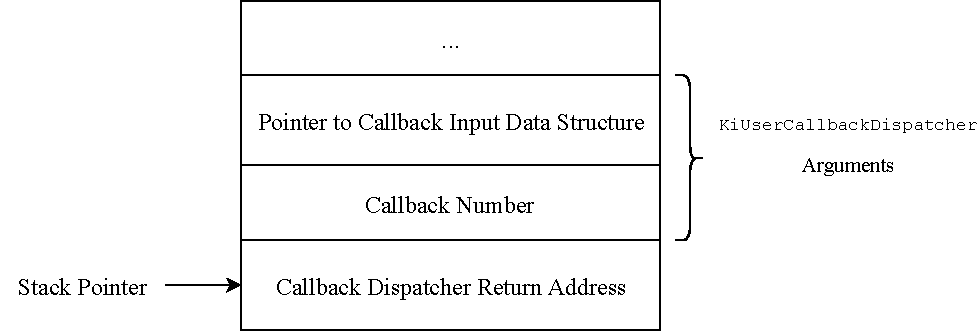
\includegraphics[width=1\textwidth]{Figures/StackCallback.pdf}
\caption{\textit{Stack before \texttt{KiUserCallbackDispatcher} execution}}
\end{figure}

Having this in mind, it is now possible to explain step-by-step how the tracing of callbacks takes place in BlueTracer:

\begin{enumerate}
\item The stack pointer value is retrieved. This is achieved through the use of the \texttt{PIN\_GetContextReg} API, that allows to get the value of a register in the context provided as input. Such context, in our specific case, is the application's register state after the context change, which, as previously mentioned, is passed as argument to the \texttt{CONTEXT\_CHANGE\_CALLBACK} notification function.
\item The callback number is obtained by adding 4 to the stack pointer and fetching the pointed value, in accordance to \textit{Figure 3.6}.
\item The \texttt{KernelCallbackTable} is retrieved from the PEB. 
\item The function pointer stored in the \texttt{KernelCallbackTable} entry indicated by the callback number is acquired.
\item It is checked if the address of the function falls within \texttt{User32.dll} memory address range. In fact, in \texttt{Win32} user mode callbacks are employed exclusively by \texttt{User32.dll} for windowing related aspects \cite{UCDispatcher}, meaning that the retrieved function address must belong to \texttt{User32.dll}'s memory address range. Such range is determined by retrieving an handle for \texttt{User32.dll} through \texttt{GetModuleHandle}, building an \texttt{IMG} object from it utilizing Pin's \texttt{IMG\_FindByAddress} and invoking the usual \texttt{IMG\_LowAddress} and \texttt{IMG\_HighAddress} functions. 
\item The name of the callback is determined by creating a \texttt{RTN} object from the function address via \texttt{RTN\_FindByAddress} and consequently invoking \texttt{RTN\_Name} on such object.
\item The callback occurrence and the callback name is recorded in the log.
\end{enumerate}

The result of the aforementioned callback tracing procedure is a log entry having the following format (\textit{Listing 3.16}).
\\
\lstset{
    language=C++,
    frame=single, % draw a frame at the top and bottom of the code block
    tabsize=4, % tab space width
    showstringspaces=false, % don't mark spaces in strings
    numbers=none, % display line numbers on the left
    commentstyle=\color{ao}, % comment color
    keywordstyle=\color{blue}, % keyword color
    stringstyle=\color{red}, % string color
    basicstyle=\footnotesize\ttfamily,
    basewidth = {.48em}
}
\begin{lstlisting}[caption={Log entry relative to a user mode callback},captionpos=b]
Context change caused by callback -> USER32.dll!LoadMenuW
\end{lstlisting}
\lstset{
    language=C++,
    frame=tb, % draw a frame at the top and bottom of the code block
    tabsize=4, % tab space width
    showstringspaces=false, % don't mark spaces in strings
    numbers=left, % display line numbers on the left
    commentstyle=\color{ao}, % comment color
    keywordstyle=\color{blue}, % keyword color
    stringstyle=\color{red}, % string color
    basicstyle=\footnotesize\ttfamily,
    basewidth = {.48em}
}


\subsection{Windows Asynchronous Procedure Calls Tracing}

\iffalse
Windows Asynchronous Procedure Calls (APCs) are employed to ... .
They are used for ...
A specific type is user-mode APCs.

A user mode APC invocation involves APCDispatcher. where the argument is the address of the function.
\fi

Windows Asynchronous Procedure Calls (APCs) are employed to alter a thread's ordinary execution path and reroute it to execute some other code. An important concept related to APCs is that, every time an APC is scheduled, it is intended for a specific thread.

APCs are utilized in many situations. Some examples are:

\begin{itemize}
\item The I{\textbackslash}O Manager employs an APC to terminate an I{\textbackslash}O operation inside the thread which started it.
\item There exists a particular APC which is used to forcibly enter in a process' execution when it has to terminate.
\item Some APIs, like \texttt{ReadFileEx} and \texttt{WriteFileEx}, utilize APCs when performing asynchronous I{\textbackslash}O operations.   
\end{itemize} 

APCs are of different types, one of which is user mode APCs. These usually call user mode code and are normally dispatched when the thread willingly enters into an alertable state. This means that, typically, user mode APCs do not asynchronously force themselves into the targeted thread, but they can be seen more like a set of work items in a queue, which the thread processes when he decides to do so \cite{APC1}.

Just like \texttt{KiUserCallbackDispatcher} for user mode callbacks, APCs are channelled by means of a single dispatcher function inside \texttt{ntdll}, named \texttt{KiUserApcDispatcher}. Such function receives as input a set of paramaters, including the address of the APC routine to be invoked and the references to two data structures in which the APC's arguments are stored \cite{APC2}.  
 
If a user mode APC takes place, in Pin the registered \texttt{CONTEXT\_CALLBACK\_NOTIFICATION} function is called immediately before the execution of \texttt{KiUserApcDispatcher}, with the reason parameter, this time, set to \texttt{CONTEXT\_CHANGE\_REASON\_APC}. Therefore, the course of action taken by BlueTracer to record user mode APCs is exactly the same as the ones for user mode callbacks, i.e. tracing the APC occurrence as well as the name of the APC that is about to be executed. Once again, however, BlueTracer does not yet support arguments' tracing in this scenario since, also in this case, the arguments are packed in data structures.

Let us now go through the steps employed by BlueTracer to trace user mode APCs:
\begin{enumerate}
\item The stack pointer value is retrieved, exactly in the same way as explained for user mode callbacks in section 3.5.1
\item The address of the APC to be invoked is obtained by adding 4 to the stack pointer and fetching the pointed value. In fact, in the stack, the APC address is located right on top of the APC's dispatcher return address, which is pointed by the stack pointer.
\item Given the address of the APC to be invoked, the corresponding \texttt{RTN} object is created via \texttt{RTN\_FindByAddress}. Similarly, from the APC address, the \texttt{IMG} object representing the DLL exporting the APC is also built, this time through the use of \texttt{IMG\_FindByAddress}.
\item The APC name and the DLL name are determined by invoking \texttt{RTN\_Name} and \texttt{IMG\_Name} respectively on the objects created in the previous step.
\item The APC-related data is recorded in the log. This includes the APC occurrence, the name of the DLL exporting the APC and the APC name. 
\end{enumerate}
 
The resulting log format is exactly the same as the one adopted for user mode callbacks. 
 
\iffalse
\section{Tool Configuration}
\fi

% !TEX root = LMThesisNicchi.tex

\chapter{Experimental Evaluation} \label{results}

In this chapter we will illustrate the results obtained during the experimental evaluation of BlueTracer.

We first tested the tool on a set of benign applications performing different tasks, in order to assess its run-time overhead. Then, we validated BlueTracer using \textit{Al-Khaser} \cite{AlK}, a popular open-source project employed to assess how stealthy a malware analysis system is with respect to a large portion of public evasion techniques used by real malware families. Finally, we employed BlueTracer to analyze a group of highly-evasive real malware samples collected by Joe Security \cite{JoeBox}, the proclaimed technology leader for the analysis of evasive malware.

\iffalse
If JoeBox added differentiate machines
\fi
The tests on benign applications and on \textit{Al-Khaser} were conducted on a VirtualBox (version 5.2.6)  Virtual Machine with 1 CPU core and 3 GB of RAM running Windows 7 32-bit, where the specifications of the host machine are:
\begin{itemize}
\item \textbf{Operating System:} Linux Mint 17.3 
\item \textbf{Processor:} Intel Core i7-3537U CPU @ 2.00 GHz $\times$ 2
\item \textbf{RAM:} 8 GB  
\end{itemize}

Instead, the tests on real malware instances were performed on a VirtualBox (version 5.2.0)  Virtual Machine with 4 CPU cores and 3 GB of RAM running Windows 7 32-bit, where the specifications of the host machine are:
\begin{itemize}
\item \textbf{Operating System:} Debian Wheezy 7 
\item \textbf{Processor:} Intel Xeon E5-4610 v2 CPU @ 2.3 GHz
\item \textbf{RAM:} 128 GB  
\end{itemize}
 

\section{Run-Time Overhead Assessment}

In order to evaluate the run-time overhead introduced by BlueTracer we tested it with a number of benign applications exercising a large number of functions. We had to perform this kind of test on deterministic batch programs to obtain accurate results rather than on real malware samples. This because malware instances have unpredictable behaviour, thus rendering the execution times obtained when running them meaningless.
Having in mind the goal of experimenting with a wide range of different functionalities, we picked a set of well-known Windows applications performing a variety of jobs. We grouped these applications based on the task they carry out, as shown below:

\begin{itemize}
\item \textbf{Collection of system information}
	   \begin{itemize}
	   \item \texttt{Systeminfo.} It outputs a summary of OS-environment parameters. 
	   \item \texttt{System File Checker (SFC).} It scans for corruptions in system files.
	   \item \texttt{Check Disk}. It checks the disks' integrity.
	   \item \texttt{IPConfig}. It displays TCP/IP network configuration values.
	   \item \texttt{Netstat}. It can show active TCP connections as well as TCP and UDP ports on which the computer is listening.
	   \item \texttt{Driver Query}. It presents the list of installed drivers and their properties.
	   \item \texttt{Windows Assessment Tools (WinSAT).} It  measures a number of performance characteristics and reports them.
	   \item \texttt{Powercfg.} It enables to search for common energy-efficiency problems. 
	   \end{itemize}
\item \textbf{Compression programs}
		\begin{itemize}
		\item \texttt{7zip.} Its default output extension is \texttt{.7z}.
		\item \texttt{IZArc.} Its default output extension is \texttt{.zip}.
		\item \texttt{WinRar.} Its default output extension is \texttt{.rar}.
		\end{itemize}
\item \textbf{Encryption Utilities}
		\begin{itemize}
		\item \texttt{Cipher.} It uses Encrypting File System (ESF), based on DESX. 
		\item \texttt{OpenSSL.} It was configured to employ 256-bit CBC AES.
		\item \texttt{Crypt.} It adopts RC2 block encryption.
		\end{itemize}
\item \textbf{Hashing Utilities}
		\begin{itemize}
		\item \texttt{File Checksum Integrity Verifier (FCIV).} It was set to use both MD5 and SHA1.
		\item \texttt{TurboSFV.} It was configured to adopt SHA3-224. 
		\end{itemize}
\end{itemize}

We first recorded the native execution time for each of the aforementioned applications. Then, we ran them under BlueTracer, logging the respective execution times. Specifically, the following BlueTracer modes of operation were employed:

\begin{itemize}
\item \textbf{Empty Image.} All image notification functions are empty, that is, they just increase a global counter value. This means that no analysis routines are inserted at run-time. 
\item \textbf{Empty Routine.} All analysis routines are empty, i.e., all they do is, once again, increase a global counter value. So, here, with respect of \textbf{Empty Image}, there is an additional cost instrumentation cost derived from the insertion of analysis routines, which collect data but do not analyze it.  
\item \textbf{Main Image.} Only Native APIs and APIs being directly invoked from the main executable of the pinned application are traced. This is BlueTracer's default mode of operation. 
\item \textbf{Complete.} Every event is traced, also including Native APIs and APIs being invoked outside the main executable (e.g., within libraries).
\end{itemize}

We tested every benign application in the previous page adopting each of the above operation modes, which can be set using BlueTracer's configuration file. Essentially, \textbf{Empty Image} and \textbf{Empty Routine} were utilized to determine the run-time overhead introduced just by the Pin's framework, when no analysis is actually performed. On the contrary, \textbf{Main Image} was adopted to show BlueTracer's overhead during a typical use of the tool, as \textbf{Main Image} is BlueTracer's default mode. Lastly, \textbf{Complete} was employed to determine how BlueTracer's behaves under heavy stress conditions.

We tested each application three times and then recorded the average execution time. For the compression programs, the file being compressed was the Puppy Linux ISO (\texttt{xenialpup-7.5-uefi.iso}), of size 332 MBs. On the other hand, for the encryption and hashing utilities, we used the Ubuntu 18.04 ISO (\texttt{ubuntu-18.04-desktop-amd64}), the size of which is 1.8 GB. During the tests, we also decided to stop the execution of the pinned application if, after it had been running for more than 10 minutes, the log file was greater than 5 GB. This had to be done due to the hard drive limitations of the testing platform.      

The recorded execution times can be observed in \textit{Table 4.1}. As the reader can see, as more demanding modes of operation are employed, the running time increases, although the increment is not uniform, but is actually quite variable across the different applications.

In light of this, to actually quantify the run-time overhead we decided to adopt the following metric:
\vspace{-0.1cm}
\begin{align*}
\text{Overhead per Event} = \frac{T_{instrumented} - T_{native}}{Events}
\end{align*}

where:
\begin{itemize}
\item $T_{instrumented}$ is the application's execution time when executed under BlueTracer with the \textbf{Complete} mode of operation enabled. We chose the \textbf{Complete} mode of operation to quantify the overhead per event in the worst-case situation.
\item $T_{native}$ is the application's native execution time.
\item $Events$ is the total number of Native API and API calls performed by the analyzed application.
\end{itemize}

\textit{Table 4.2} lists the overhead per event value of each benign application for which the execution time in the \textbf{Complete} mode of operation could be obtained. In this case we can see that the typical overhead is approximately in the range of 40 - 220 microseconds per operation, with the compression programs being an exception, as they have a greater overhead per event value than the rest.

%\vspace*{0.8cm}
\begin{sidewaystable}
\centering
%\begin{tabular}{cccccc}
\newcolumntype{Y}{>{\centering\arraybackslash}X}
\newcommand{\specialcell}[2][c]{%
  \begin{tabular}[#1]{@{}c@{}}#2\end{tabular}}
\begin{tabularx}{\linewidth}{*{6}{Y}}

\hline
\hline
   \textbf{Application} & \specialcell{ \textbf{Native} \\ \textbf{(s)}} & \specialcell{ \textbf{Empty Image} \\ \textbf{(s)}} & \specialcell{ \textbf{Empty Routine} \\ \textbf{(s)}} & \specialcell{ \textbf{Main Image} \\ \textbf{(s)}} & \specialcell{ \textbf{Complete} \\ \textbf{(s)}} \\
\hline
\texttt{Systeminfo}      & 5.894    & 9.686 (1.64x)  & 12.869 (2.18x) & 15.694 (2.66x) & 26.398 (4.48x)     \\
\texttt{SFC}          & 218.251 & 222.065 (1.02x) & 226.125 (1.04x) & 230.869 (1.06x) & 245.476 (1.12x)       \\
\texttt{Check Disk}       & 101.570     & 171.94 (1.69x) & 181.429 (1.79x) & 454.649 (4.48x) & 600+       \\
\texttt{IPConfig}       & 0.105     & 4.257 (40.54x) & 8.421 (80.20x) & 9.599 (91.42x) & 13.181 (125.53x)      \\
\texttt{Netstat} & 0.085 & 2.563 (30.15x) & 4.630 (54.47x) & 6.902 (81.20x) & 21.129 (248.58x)       \\
\texttt{DriverQuery} & 1.168 & 6.663 (5.70x) & 9.786 (8.38x) & 34.074 (29.17x) & 68.668 (58.79x)     \\
\texttt{WinSat}       & 163.175     & 212.496 (1.30x) & 221.012 (1.35x) & 273.641 (1.68x) & 600+      \\
\texttt{PowerCFG} & 61.333      & 73.325 (1.20x) & 80.018 (1.30x) & 132.466 (2.16x) & 273.882 (4.47x)       \\
\texttt{7zip}       & 175.526     & 212.000 (1.21x) & 225.091 (1.28x) & 227.985 (1.30x) & 233.792 (1.33x)      \\
\texttt{IZArc}      & 30.920     & 52.878 (1.71x) & 56.631 (1.83x) & 61.066 (1.97x) & 65.770 (2.13x)      \\
\texttt{WinRar} & 155.674 & 192.638 (1.24x) & 198.804 (1.28x) & 208.606 (1.34x) & 215.455 (1.38x)      \\
\texttt{Cipher} & 0.028 & 1.817 (64.89x) & 3.787 (135.25x) & 4.435 (158.39x) & 5.064 (180.86x)       \\
\texttt{OpenSSL} & 24.769 & 33.183 (1.34x) & 34.308 (1.39x) & 47.006 (1.90x) & 1524.763 (61.56x)      \\
\texttt{Crypt} & 65.392 & 140.048 (2.14x) & 142.979 (2.19x) & 572.353 (8.75x) & 600+      \\
\texttt{FCIV} & 10.807 & 25.113 (2.32x) & 28.144 (2.60x) & 56.329 (5.21x) & 87.948 (8.14x)       \\
\texttt{TurboSFV} & 34.412 & 57.705 (1.68x) & 62.639 (1.82x) & 66.439 (1.93x) & 74.657 (2.17x)
\\
\hline
\end{tabularx}
\vspace{0.2cm}
\caption{Execution times of instrumented benign applications}

\end{sidewaystable}

\iffalse
\begin{table}
\centering
%\begin{tabular}{cccccc}
\newcolumntype{Y}{>{\centering\arraybackslash}X}
\newcommand{\specialcell}[2][c]{%
  \begin{tabular}[#1]{@{}c@{}}#2\end{tabular}}
\begin{tabularx}{\linewidth}{*{4}{Y}}
\hline
\hline
\cline{1-2}
   \textbf{Application} & \specialcell{ \textbf{Complete} \\ \textbf{(s)}} & \textbf{Events} & \specialcell{ \textbf{Overhead / Event} \\ \textbf{(s)}} \\
\hline
\texttt{Systeminfo}      & 26.398    & 387 476      \\
\texttt{System File Checker}          & each        & 0.01       \\
\texttt{Check Disk}       & stuffed     & 92.50      \\
\texttt{IPConfig}       & stuffed     & 33.33      \\
\texttt{Netstat} & frozen      & 8.99       \\
\texttt{DriverQuery}       & stuffed     & 92.50      \\
\texttt{WinSat}       & stuffed     & 33.33      \\
\texttt{PowerCFG} & frozen      & 8.99       \\
\texttt{7zip}       & stuffed     & 92.50      \\
\texttt{IZArc}      & stuffed     & 33.33      \\
\texttt{WinRar} & frozen      & 8.99       \\
\texttt{Cipher} & frozen      & 8.99       \\
\texttt{OpenSSL}       & stuffed     & 92.50      \\
\texttt{Crypt}      & stuffed     & 33.33      \\
\texttt{FCIV} & frozen      & 8.99       \\
\hline
\end{tabularx}
\caption{Run-time overhead for benign applications}
\end{table}
\fi

\vspace*{0.8cm}
\begin{sidewaystable}
\centering
%\begin{tabular}{cccccc}
\newcolumntype{Y}{>{\centering\arraybackslash}X}
\newcommand{\specialcell}[2][c]{%
  \begin{tabular}[#1]{@{}c@{}}#2\end{tabular}}
\begin{tabularx}{\linewidth}{*{6}{Y}}

\hline
\hline
   \textbf{Application} & \specialcell{ \textbf{Native} \\ \textbf{(s)}} & \specialcell{ \textbf{Complete} \\ \textbf{(s)}} & \textbf{Events} & \specialcell{ \textbf{Overhead per Event} \\  \textbf{($10^-5$ s)} }  \\
\hline
\texttt{Systeminfo}      & 5.894    & 26.398  & 387 476 & $5.291$    \\
\texttt{SFC}          & 218.251 & 245.476 & 333 781 & $8.156$ \\
\texttt{IPConfig}       & 0.105 & 13.181 & 94 313 & $13.864$      \\
\texttt{Netstat} & 0.085 & 21.129 & 542 649 & $3.878$       \\
\texttt{DriverQuery} & 1.168 & 68.668 & 1 735 859 & $3.860$            \\
\texttt{PowerCFG} & 61.333 & 273.882 & 4 497 247 & $4.726$       \\
\texttt{7zip}       & 175.526 & 233.792 & 146 578 & $39.751$      \\
\texttt{IZArc}      & 30.920 & 65.770 & 109 142 & $31.931$      \\
\texttt{WinRar} & 155.674 & 215.455 & 84 329 & $70.890$      \\
\texttt{Cipher} & 0.028 & 4.435 & 24 141 & $18.255$           \\
\texttt{OpenSSL} & 24.769 & 1524.763 & 57 410 809 & $2.613$                \\
\texttt{FCIV} & 10.807 & 87.948 & 725 133 &  $10.638$               \\
\texttt{TurboSFV} & 34.412 & 74.657 & 183 455 & $21.937$ 
\\
\hline
\end{tabularx}
\vspace{0.2cm}
\caption{Run-time overhead for benign applications}

\end{sidewaystable}

\vspace{-1cm}
\section{Al-Khaser} \label{Alk}
Al-Khaser \cite{AlK} is a popular open-source application which performs a large number of common checks employed by malware families to determine if they are being executed in an analysis environment. It is typically utilized to assess how stealthy and well hidden a malware analysis system is. For this reason, we chose Al-Khaser as our main validation tool.

The checks implemented by Al-Khaser are divided into categories, with the most significant ones being the following:
\begin{itemize}
\item \textbf{Anti-Debugging}, aimed at detecting the presence of a debugger.
\item \textbf{Anti-Sandbox Timing-based}, the purpose of which is to let sandboxes time out in order to defy analysis. 
\item \textbf{Human Interaction Detection}, which seek to discover the presence of a sandbox by looking for the lack of human interaction with the system.
\item \textbf{Anti-Virtualization}, which have the objective of exposing the use of virtualization and full-system emulation. 
\item \textbf{Anti-Analysis}, aimed at uncovering the employment of common analysis tools (e.g OllyDbg, IDA Pro, etc. ).
\end{itemize}  

When Al-Khaser's executable is run, all the checks are performed and the outcome of each one of them can be easily observed from the command line: \texttt{GOOD} is printed if the analysis product succeeded at remaining hidden, and \texttt{BAD} otherwise. 

To validate BlueTracer, Al-Khaser was run under it in the default \textbf{Main Image} mode. The result was that BlueTracer managed to remain undetected thanks to its integration with BluePill with respect to all the checks performed by Al-Khaser. From this outcome we obtained a first confirmation of BlueTracer's ability to hide its presence. 

Furthermore, to also validate BlueTracer's tracing power, we analyzed the logs obtained when running Al-Khaser, with the objective of finding evidence of the performed evasion checks.
Even in this case, BlueTracer performed well, as the checks could easily be deduced from the log file. 

Let us now show how some of these checks appeared on the log, in order to give a better idea of what BlueTracer is capable of. To be as clear as possible, we will use the same checks categorization as Al-Khaser's.

\subsubsection*{Anti-Debugging}

Anti-debugging checks are essentially aimed at determining if a program is running under a debugger. As already mentioned in Section~\ref{Debugger}, there exist Windows APIs whose objective is exactly to discover if the calling process is being debugged.
A well-known API of this kind is \texttt{IsDebuggerPresent}, which returns a nonzero value if the calling process is running in the context of a debugger and zero otherwise. Such API is employed in one of Al-Khaser's anti-debugging checks and is properly recorded by BlueTracer (\textit{Listing 4.1}). As the reader can see below, the return value is zero, as no debugger is detected.

\vspace{0.5cm}
\lstset{
    language=C++,
    frame=tb, % draw a frame at the top and bottom of the code block
    tabsize=4, % tab space width
    showstringspaces=false, % don't mark spaces in strings
    numbers=none, % display line numbers on the left
    commentstyle=\color{ao}, % comment color
    keywordstyle=\color{blue}, % keyword color
    stringstyle=\color{red}, % string color
    basicstyle=\footnotesize\ttfamily,
    basewidth = {.48em}
}
\begin{lstlisting}[caption={Log entry relative to \texttt{IsDebuggerPresent}},captionpos=b]
~~3160~~ 562 kernel32.dll!IsDebuggerPresent
~~3160~~ 563 KERNELBASE.dll!IsDebuggerPresent
563    executed KERNELBASE.dll!IsDebuggerPresent =>
563 	retval: 0x0 (name=Return value, type=(long/int), size=0x4)
\end{lstlisting}
\lstset{
    language=C++,
    frame=tb, % draw a frame at the top and bottom of the code block
    tabsize=4, % tab space width
    showstringspaces=false, % don't mark spaces in strings
    numbers=left, % display line numbers on the left
    commentstyle=\color{ao}, % comment color
    keywordstyle=\color{blue}, % keyword color
    stringstyle=\color{red}, % string color
    basicstyle=\footnotesize\ttfamily,
    basewidth = {.48em}
}

Another popular Windows API for debug detection is \texttt{CheckRemoteDebuggerPresent}, which determines if the specified process is being debugged by a "remote" debugger, i.e., a debugger residing in parallel and different process.
Its second argument is a pointer to a boolean, which is set to true if the provided process is being debugged, or false otherwise. Al-Khaser also adopts this API, and, again, BlueTracer correctly logged its invocation (\textit{Listing 4.2}). In addition, it is worth noting that the output value for the second argument (\texttt{arg 1}) is 
false (\texttt{0x0}), thus showing once more that a debugger was not discovered.

\vspace{0.5cm}
\lstset{
    language=C++,
    frame=tb, % draw a frame at the top and bottom of the code block
    tabsize=4, % tab space width
    showstringspaces=false, % don't mark spaces in strings
    numbers=none, % display line numbers on the left
    commentstyle=\color{ao}, % comment color
    keywordstyle=\color{blue}, % keyword color
    stringstyle=\color{red}, % string color
    basicstyle=\footnotesize\ttfamily,
    basewidth = {.48em}
}
\begin{lstlisting}[caption={Log entry relative to \texttt{CheckRemoteDebuggerPresent}},captionpos=b]
~~3160~~ 1450 kernel32.dll!CheckRemoteDebuggerPresent
1450 	arg 0: 0xffffffff (name=hProcess, type=DWORD, size=0x4)
1450 	arg 1: 0x002bf710 => 0x0 (name=pbDebuggerPresent, type=(long/int)*, size=0x4)
1450    executed kernel32.dll!CheckRemoteDebuggerPresent =>
1450 	arg 1: 0x002bf710 => 0x0 (name=pbDebuggerPresent, type=(long/int)*, size=0x4)
1450 	retval: 0x1 (name=Return value, type=(long/int), size=0x4)
\end{lstlisting}
\lstset{
    language=C++,
    frame=tb, % draw a frame at the top and bottom of the code block
    tabsize=4, % tab space width
    showstringspaces=false, % don't mark spaces in strings
    numbers=left, % display line numbers on the left
    commentstyle=\color{ao}, % comment color
    keywordstyle=\color{blue}, % keyword color
    stringstyle=\color{red}, % string color
    basicstyle=\footnotesize\ttfamily,
    basewidth = {.48em}
}   

Debugger detection is not only achieved through the use of Windows APIs. In fact, there are also some Native APIs which can be used for this purpose. One of them is \texttt{NtQueryInformationProcess}, which retrieves information related to the specified process. Its second parameter is utilized to specify the type of process information to be retrieved. When set to \texttt{ProcessDebugPort} (value \texttt{0x7}), the Native API provides information on whether the supplied process is being debugged. Specifically, if a debugger is present, the \texttt{ProcessInformation} output parameter is set to a non-zero port number, while, if the process is not under a debugger, this parameter is set to zero \cite{Sikorski:2012:PMA:2181153}. Al-Khaser performs this check and, once more, BlueTracer recorded it (\textit{Listing 4.3}).

\vspace{0.5cm}
\lstset{
    language=C++,
    frame=tb, % draw a frame at the top and bottom of the code block
    tabsize=4, % tab space width
    showstringspaces=false, % don't mark spaces in strings
    numbers=none, % display line numbers on the left
    commentstyle=\color{ao}, % comment color
    keywordstyle=\color{blue}, % keyword color
    stringstyle=\color{red}, % string color
    basicstyle=\footnotesize\ttfamily,
    basewidth = {.48em}
}
\begin{lstlisting}[caption={Log entry relative to \texttt{NtQueryInformationProcess}},captionpos=b]
~~3160~~ 3186 ntdll.dll!NtQueryInformationProcess
3186 	arg 0: 0xffffffff (type=HANDLE, size=0x4)
3186 	arg 1: 0x7 (type=int, size=0x4)
3186 	arg 2: 0x002bf6cc (type=<struct>*, size=0x4)
3186 	arg 3: 0x0 (type=unsigned int, size=0x4)
3186 	arg 4: 0x003c0e98 (type=unsigned int*, size=0x4)
3186    succeeded =>
3186 	arg 2: 0x002bf6cc (type=<struct>*, size=0x4)
3186 	arg 4: 0x003c0e98 => 0x3c0ea0 (type=unsigned int*, size=0x4)
3186 	retval: 0x0 (type=NTSTATUS, size=0x4
\end{lstlisting}
\lstset{
    language=C++,
    frame=tb, % draw a frame at the top and bottom of the code block
    tabsize=4, % tab space width
    showstringspaces=false, % don't mark spaces in strings
    numbers=left, % display line numbers on the left
    commentstyle=\color{ao}, % comment color
    keywordstyle=\color{blue}, % keyword color
    stringstyle=\color{red}, % string color
    basicstyle=\footnotesize\ttfamily,
    basewidth = {.48em}
}  

In particular, it can be deduced from \texttt{arg 1}'s value that \texttt{ProcessDebugPort} is adopted. Unfortunately, this time, we cannot tell from the log that a debugger has not been detected because the output paramater containing this information (\texttt{arg 2}) is a pointer to a \texttt{struct}, which changes based on the type of process information requested. BlueTracer does not yet address these complex cases and we are planning to address them in future versions of the tool.  

\subsubsection*{Anti-Sandbox Timing-based}

Anti-sandbox timing-based checks have the objective of hindering dynamic analysis by making sandboxes time out and, in some cases, they also measure the time elapsed between sleep operations to detect time fast-forwarding strategies. Luckily, BluePill \cite{BluePill} addresses these checks by adopting a sophisticated strategy based on manipulating the timer behaviour of a process. This means that BlueTracer can record timing-based checks without worrying about being detected.

The \texttt{NtDelayExecution} Native API is the lowest level user mode mechanism which can be employed to suspend execution. It takes as input two paramaters: a boolean that makes the Native API alertable when set to \texttt{true} and a \texttt{LARGE\_INTEGER} defining the delay interval. If the value for the second parameter is negative, it specifies the \textit{relative} amount to sleep in units of 100 nanoseconds; otherwise, it indicates an \textit{absolute time}, i.e., the date and time when to stop sleeping. Al-Khaser makes use of this Native API and BlueTracer was able to correctly trace it (\textit{Listing 4.4}). In particular, from the log entry, it can be seen that a negative delay was specified, meaning that a \textit{relative} time to sleep was provided.  

\vspace{0.5cm}
\lstset{
    language=C++,
    frame=tb, % draw a frame at the top and bottom of the code block
    tabsize=4, % tab space width
    showstringspaces=false, % don't mark spaces in strings
    numbers=none, % display line numbers on the left
    commentstyle=\color{ao}, % comment color
    keywordstyle=\color{blue}, % keyword color
    stringstyle=\color{red}, % string color
    basicstyle=\footnotesize\ttfamily,
    basewidth = {.48em}
}
\begin{lstlisting}[caption={Log entry relative to \texttt{NtDelayExecution}},captionpos=b]
~~3160~~ 46332 ntdll.dll!NtDelayExecution
46332 	arg 0: 0x0 (type=bool, size=0x1)
46332 	arg 1: 0xffffffff4d2fa200(hex) (type=LARGE_INTEGER*, size=0x4)
46332    succeeded =>
46332 	retval: 0x0 (type=NTSTATUS, size=0x4)
\end{lstlisting}
\lstset{
    language=C++,
    frame=tb, % draw a frame at the top and bottom of the code block
    tabsize=4, % tab space width
    showstringspaces=false, % don't mark spaces in strings
    numbers=left, % display line numbers on the left
    commentstyle=\color{ao}, % comment color
    keywordstyle=\color{blue}, % keyword color
    stringstyle=\color{red}, % string color
    basicstyle=\footnotesize\ttfamily,
    basewidth = {.48em}
}   

\texttt{WaitForSingleObject} is also often used to wait until a time-out interval elapses. In input, it receives an handle to an object and a time-out interval in milliseconds. Then, it waits until the provided object is in the signaled state or the time-out runs out. Al-Khaser also adopts this API in its set of timing-based checks. Once more, BlueTracer was capable of recording its occurrence (\textit{Listing 4.5}). It is relevant to point out that the return value is \texttt{0x102}, which indicates that the API has returned because the time-out interval has elapsed, just as expected.

\vspace{0.5cm}
\lstset{
    language=C++,
    frame=tb, % draw a frame at the top and bottom of the code block
    tabsize=4, % tab space width
    showstringspaces=false, % don't mark spaces in strings
    numbers=none, % display line numbers on the left
    commentstyle=\color{ao}, % comment color
    keywordstyle=\color{blue}, % keyword color
    stringstyle=\color{red}, % string color
    basicstyle=\footnotesize\ttfamily,
    basewidth = {.48em}
}
\begin{lstlisting}[caption={Log entry relative to \texttt{WaitForSingleObject}},captionpos=b]
~~3160~~ 50077 kernel32.dll!WaitForSingleObject
50077 	arg 0: 0x204 (name=hHandle, type=DWORD, size=0x4)
50077 	arg 1: 0x493e0 (name=dwMilliseconds, type=DWORD, size=0x4)
50077    executed kernel32.dll!WaitForSingleObject =>
50077 	retval: 0x102 (name=Return value, type=DWORD, size=0x4)
\end{lstlisting}
\lstset{
    language=C++,
    frame=tb, % draw a frame at the top and bottom of the code block
    tabsize=4, % tab space width
    showstringspaces=false, % don't mark spaces in strings
    numbers=left, % display line numbers on the left
    commentstyle=\color{ao}, % comment color
    keywordstyle=\color{blue}, % keyword color
    stringstyle=\color{red}, % string color
    basicstyle=\footnotesize\ttfamily,
    basewidth = {.48em}
} 

The most well-known API for suspending execution is surely \texttt{sleep}, that simply takes as input the number of milliseconds for which execution is to be delayed.

\vspace{0.5cm}
\lstset{
    language=C++,
    frame=tb, % draw a frame at the top and bottom of the code block
    tabsize=4, % tab space width
    showstringspaces=false, % don't mark spaces in strings
    numbers=none, % display line numbers on the left
    commentstyle=\color{ao}, % comment color
    keywordstyle=\color{blue}, % keyword color
    stringstyle=\color{red}, % string color
    basicstyle=\footnotesize\ttfamily,
    basewidth = {.48em}
}
\begin{lstlisting}[caption={Portion of \texttt{Sleep} loop },captionpos=b]
~~3160~~ 9225 kernel32.dll!Sleep
9225 	arg 0: 0xf (name=dwMilliseconds, type=DWORD, size=0x4)
~~3160~~ 9226 KERNELBASE.dll!Sleep
9226 	arg 0: 0xf (name=dwMilliseconds, type=DWORD, size=0x4)
9226    executed KERNELBASE.dll!Sleep =>
9226 	retval: 0x00000000 (name=Return value, type=void, size=0x0)
~~3160~~ 9227 ntdll.dll!NtYieldExecution
9227    failed (error=0x40000024) =>
9227 	retval: 0x40000024 (type=NTSTATUS, size=0x4)
~~3160~~ 9228 kernel32.dll!Sleep
9228 	arg 0: 0xf (name=dwMilliseconds, type=DWORD, size=0x4)
~~3160~~ 9229 KERNELBASE.dll!Sleep
9229 	arg 0: 0xf (name=dwMilliseconds, type=DWORD, size=0x4)
9229    executed KERNELBASE.dll!Sleep =>
9229 	retval: 0x00000000 (name=Return value, type=void, size=0x0)
~~3160~~ 9230 ntdll.dll!NtYieldExecution
9230    failed (error=0x40000024) =>
9230 	retval: 0x40000024 (type=NTSTATUS, size=0x4)
\end{lstlisting}
\lstset{
    language=C++,
    frame=tb, % draw a frame at the top and bottom of the code block
    tabsize=4, % tab space width
    showstringspaces=false, % don't mark spaces in strings
    numbers=left, % display line numbers on the left
    commentstyle=\color{ao}, % comment color
    keywordstyle=\color{blue}, % keyword color
    stringstyle=\color{red}, % string color
    basicstyle=\footnotesize\ttfamily,
    basewidth = {.48em}
}   

Due to its popularity, Al-Khaser had to adopt it and, again, BlueTracer's logs showed evidence of its usage (\textit{Listing 4.6}). Specifically, from the log file, it can be deduced that \texttt{sleep} was used in a loop, as it is invoked many times subsequently.

\subsubsection*{Human Interaction Detection}

The idea behind human interaction detection checks is to uncover the presence of a sandbox based on the lack of human interaction with the system; in fact, in real environments users typically perform some detectable activities when carrying out their tasks. A classical example of such activities is moving the mouse cursor.  

The mouse cursor position can be obtained through the use of the \texttt{GetCursorPos} API, which has a single output parameter containing a pointer to a \texttt{POINT struct}. Such data structure stores the retrieved position of the mouse cursor, in screen coordinates. Al-Khaser employs the \texttt{GetCursorPos} API to check if there is some kind of mouse movement in the sandbox. BlueTracer proved to work well as it traced the API's invocation (\textit{Listing 4.7}).

\vspace{0.5cm}
\lstset{
    language=C++,
    frame=tb, % draw a frame at the top and bottom of the code block
    tabsize=4, % tab space width
    showstringspaces=false, % don't mark spaces in strings
    numbers=none, % display line numbers on the left
    commentstyle=\color{ao}, % comment color
    keywordstyle=\color{blue}, % keyword color
    stringstyle=\color{red}, % string color
    basicstyle=\footnotesize\ttfamily,
    basewidth = {.48em}
}
\begin{lstlisting}[caption={\texttt{GetCursorPos} evidence in the log },captionpos=b]
~~3160~~ 17964 USER32.dll!GetCursorPos
17964 	arg 0: 0x002bf684 (name=lpPoint, type=struct*|tagPOINT, size=0x40)
17964    executed USER32.dll!GetCursorPos =>
17964 	arg 0: 0x002bf684 (name=lpPoint, type=struct*|tagPOINT, size=0x40)
17964 	retval: 0x1 (name=Return value, type=(long/int), size=0x4)
~~3160~~ 17965 kernel32.dll!Sleep
17965 	arg 0: 0x1388 (name=dwMilliseconds, type=DWORD, size=0x4)
~~3160~~ 17966 KERNELBASE.dll!Sleep
17966 	arg 0: 0x1388 (name=dwMilliseconds, type=DWORD, size=0x4)
17966    executed KERNELBASE.dll!Sleep =>
17966 	retval: 0x00000000 (name=Return value, type=void, size=0x0)
~~3160~~ 17967 USER32.dll!GetCursorPos
17967 	arg 0: 0x002bf698 (name=lpPoint, type=struct*|tagPOINT, size=0x40)
17967    executed USER32.dll!GetCursorPos =>
17967 	arg 0: 0x002bf698 (name=lpPoint, type=struct*|tagPOINT, size=0x40)
17967 	retval: 0x1 (name=Return value, type=(long/int), size=0x4)
\end{lstlisting}
\lstset{
    language=C++,
    frame=tb, % draw a frame at the top and bottom of the code block
    tabsize=4, % tab space width
    showstringspaces=false, % don't mark spaces in strings
    numbers=left, % display line numbers on the left
    commentstyle=\color{ao}, % comment color
    keywordstyle=\color{blue}, % keyword color
    stringstyle=\color{red}, % string color
    basicstyle=\footnotesize\ttfamily,
    basewidth = {.48em}
} 

It is interesting to notice that, from the log, it can be also deduced how the actual check is carried out by Al-Khaser. In fact, \texttt{GetCursorPos} is called, followed by a \texttt{Sleep} and another \texttt{GetCursorPos} invocation. In light of this, it is likely that an initial cursor position was first retrieved, which was later compared with the cursor position obtained after the sleep operation, with the aim of determining if the mouse cursor had moved in the mean time.
  

\subsubsection*{Anti-Virtualization}
Anti-virtualization checks look for a number of artifacts in the guest operating system introduced by hypervisors which are specific to virtual machines.

A common way to detect virtualization is by checking Windows registry artifacts. The Windows registry is a hierarchical tree-like database containing critical data for both the Windows operating system and its applications. Each node of the tree is a \textit{key} and every key embodies \textit{subkeys} and \textit{values} \cite{Regs}. 

\vspace{0.5cm}
\lstset{
    language=C++,
    frame=tb, % draw a frame at the top and bottom of the code block
    tabsize=4, % tab space width
    showstringspaces=false, % don't mark spaces in strings
    numbers=none, % display line numbers on the left
    commentstyle=\color{ao}, % comment color
    keywordstyle=\color{blue}, % keyword color
    stringstyle=\color{red}, % string color
    basicstyle=\footnotesize\ttfamily,
    basewidth = {.48em}
}
\begin{lstlisting}[caption={Log entry relative to \texttt{RegOpenKeyExW} },captionpos=b]
~~3160~~ 30134 ADVAPI32.dll!RegOpenKeyExW
30134 	arg 0: 0x80000002 (name=hKey, type=DWORD, size=0x4)
30134 	arg 1: HARDWARE\ACPI\DSDT\VBOX__ (name=lpSubKey, type=wchar_t*, size=0x2)
30134 	arg 2: 0x0 (name=ulOptions, type=DWORD, size=0x4)
30134 	arg 3: 0x20019 (name=samDesired, type=DWORD, size=0x4)
30134 	arg 4: 0x002bf6e4 => 0x0 (name=phkResult, type=DWORD*, size=0x4)
~~3160~~ 30135 kernel32.dll!RegOpenKeyExW
30135 	arg 0: 0x80000002 (name=hKey, type=DWORD, size=0x4)
30135 	arg 1: HARDWARE\ACPI\DSDT\VBOX__ (name=lpSubKey, type=wchar_t*, size=0x2)
30135 	arg 2: 0x0 (name=ulOptions, type=DWORD, size=0x4)
30135 	arg 3: 0x20019 (name=samDesired, type=DWORD, size=0x4)
30135 	arg 4: 0x002bf6e4 => 0x0 (name=phkResult, type=DWORD*, size=0x4)
30135    executed kernel32.dll!RegOpenKeyExW =>
30135 	arg 4: 0x002bf6e4 => 0x0 (name=phkResult, type=DWORD*, size=0x4)
30135 	retval: 0x2 (name=Return value, type=(long/int), size=0x4))
\end{lstlisting}
\lstset{
    language=C++,
    frame=tb, % draw a frame at the top and bottom of the code block
    tabsize=4, % tab space width
    showstringspaces=false, % don't mark spaces in strings
    numbers=left, % display line numbers on the left
    commentstyle=\color{ao}, % comment color
    keywordstyle=\color{blue}, % keyword color
    stringstyle=\color{red}, % string color
    basicstyle=\footnotesize\ttfamily,
    basewidth = {.48em}
}

The existence of some specific registry keys is enough to reveal the presence of virtualization. For instance, the key \texttt{HKEY\_LOCAL\_MACHINE\textbackslash}\texttt{{HARDWARE}\textbackslash{ACPI}\textbackslash{DSDT}}\texttt{\textbackslash{VBOX}\textbackslash\_\_}
gives away the presence of VirtualBox. Al-Khaser looks for these kinds of Windows registry artifacts and BlueTracer is able to record such events (\textit{Listing 4.8}).

From \textit{Listing 4.8}, it can be observed that the aforementioned registry key is searched through the use of the \texttt{RegOpenKeyExW} API, which normally opens the specified registry key. However, in this case, a "file not found" error value (\texttt{0x2}) is returned since the registry key is not found, thus also confirming BlueTracer's ability to remain hidden.

In addition to Windows registry artifacts, there are also many file system artifacts which can be checked in order to uncover the presence of a virtualized environment. Typically, specific files are searched. Al-Khaser, for instance, looks for a number of files, one of which is the \texttt{VboxMouse.sys} driver of Virtualbox. Once more, BlueTracer was able to trace these file-searching events, including the ones relative to \texttt{VboxMouse.sys} (\textit{Listing 4.9}). 

\vspace{0.5cm}
\lstset{
    language=C++,
    frame=tb, % draw a frame at the top and bottom of the code block
    tabsize=4, % tab space width
    showstringspaces=false, % don't mark spaces in strings
    numbers=none, % display line numbers on the left
    commentstyle=\color{ao}, % comment color
    keywordstyle=\color{blue}, % keyword color
    stringstyle=\color{red}, % string color
    basicstyle=\footnotesize\ttfamily,
    basewidth = {.48em}
}
\begin{lstlisting}[caption={ Log portion relative to the search for \texttt{VboxMouse.sys} search},captionpos=b]
~~3160~~ 24979 kernel32.dll!GetFileAttributesW
24979 	arg 0: C:\Windows\system32\drivers\VBoxMouse.sys
 (name=lpFileName, type=wchar_t*, size=0x2)
~~3160~~ 24980 KERNELBASE.dll!GetFileAttributesW
24980 	arg 0: C:\Windows\system32\drivers\VBoxMouse.sys
 (name=lpFileName, type=wchar_t*, size=0x2)
24980    executed KERNELBASE.dll!GetFileAttributesW =>
24980 	retval: 0xffffffff (name=Return value, type=DWORD, size=0x4)
\end{lstlisting}
\lstset{
    language=C++,
    frame=tb, % draw a frame at the top and bottom of the code block
    tabsize=4, % tab space width
    showstringspaces=false, % don't mark spaces in strings
    numbers=left, % display line numbers on the left
    commentstyle=\color{ao}, % comment color
    keywordstyle=\color{blue}, % keyword color
    stringstyle=\color{red}, % string color
    basicstyle=\footnotesize\ttfamily,
    basewidth = {.48em}
} 

The \texttt{GetFileAttributesW} API, as the name suggests, is typically employed to obtain file attributes for the specified file. From \textit{Listing 4.9} it can be seen that the API returns -1, since the requested file was not found. Therefore, even in this situation, BlueTracer was also undetected.

\iffalse
-Registry Artifacts
-File system artifacts -> Virtual Devices here?
-Window
-DLLs
\fi

A virtualized environment can be also discovered by looking for specific windows. The \texttt{FindWindow} API returns an handle of a window belonging to a specific class or having the specified name. This API can be exploited to check for the presence of a window associated to a virtualization program. A typical example of this trick, which is implemented by Al-Khaser, is searching for a window named "VBoxTrayToolWnd", as the presence of such window indicates that VirtualBox is being utilized. BlueTracer also detected this check (\textit{Listing 4.10}). As the reader can see, the return value is \texttt{null}, meaning that the window was not found and that BlueTracer did not reveal its presence.

\vspace{0.5cm}
\lstset{
    language=C++,
    frame=tb, % draw a frame at the top and bottom of the code block
    tabsize=4, % tab space width
    showstringspaces=false, % don't mark spaces in strings
    numbers=none, % display line numbers on the left
    commentstyle=\color{ao}, % comment color
    keywordstyle=\color{blue}, % keyword color
    stringstyle=\color{red}, % string color
    basicstyle=\footnotesize\ttfamily,
    basewidth = {.48em}
}
\begin{lstlisting}[caption={ Log entry relative to \texttt{FindWindowW}},captionpos=b]
~~3160~~ 35247 USER32.dll!FindWindowW
35247 	arg 0: <null> (name=lpClassName, type=wchar_t*, size=0x2)
35247 	arg 1: VBoxTrayToolWnd (name=lpWindowName, type=wchar_t*, size=0x2)
35247    executed USER32.dll!FindWindowW =>
35247 	retval: 0x0 (name=Return value, type=DWORD, size=0x4)
\end{lstlisting}
\lstset{
    language=C++,
    frame=tb, % draw a frame at the top and bottom of the code block
    tabsize=4, % tab space width
    showstringspaces=false, % don't mark spaces in strings
    numbers=left, % display line numbers on the left
    commentstyle=\color{ao}, % comment color
    keywordstyle=\color{blue}, % keyword color
    stringstyle=\color{red}, % string color
    basicstyle=\footnotesize\ttfamily,
    basewidth = {.48em}
} 
   

\subsubsection{Anti-Analysis}

\iffalse
Check for processes of common anti-analysis tools
\fi

Lastly, anti-analysis checks are aimed at detecting the existence of processes belonging to popular analysis tools. One of such tools is Process Monitor (\texttt{procmon.exe}), which is an advanced Windows monitoring tool that shows real-time file system, registry and process/thread activity \cite{procmon}. Al-Khaser looks for the processes of many analysis tools, including Process Monitor. Again, BlueTracer was also able to successfully log anti-analysis events, even the ones directed at uncovering the presence of Process Monitor (\textit{Listing 4.11}). From the listing on the next page, it can be seen that the course of action adopted by Al-Khaser is quite straightforward. It first takes a snapshot of all the processes in the system with \texttt{CreateToolhelp32Snapshot}. Then, for each process in the snapshot, it retrieves the corresponding name, through the use of \texttt{Process32FirstW} at the beginning and \texttt{Process32NextW} afterwards, and compares it with \texttt{procmon.exe} via \texttt{StrCmpIW}. 
\newpage
\lstset{
    language=C++,
    frame=tb, % draw a frame at the top and bottom of the code block
    tabsize=4, % tab space width
    showstringspaces=false, % don't mark spaces in strings
    numbers=none, % display line numbers on the left
    commentstyle=\color{ao}, % comment color
    keywordstyle=\color{blue}, % keyword color
    stringstyle=\color{red}, % string color
    basicstyle=\footnotesize\ttfamily,
    basewidth = {.48em}
}
\begin{lstlisting}[caption={\texttt{procmon.exe} search},captionpos=b]
~~3160~~ 53940 kernel32.dll!CreateToolhelp32Snapshot
53940 	arg 0: 0x2 (name=dwFlags, type=DWORD, size=0x4)
53940 	arg 1: 0x0 (name=th32ProcessID, type=DWORD, size=0x4)
53940    executed kernel32.dll!CreateToolhelp32Snapshot =>
53940 	retval: 0x1fc (name=Return value, type=DWORD, size=0x4)
~~3160~~ 53941 kernel32.dll!Process32FirstW
53941 	arg 0: 0x1fc (name=hSnapshot, type=DWORD, size=0x4)
53941 	arg 1: 0x002b7408 (name=lppe, type=struct*|tagPROCESSENTRY32W, size=0x1160)
53941    executed kernel32.dll!Process32FirstW =>
53941 	arg 1: 0x002b7408 (name=lppe, type=struct*|tagPROCESSENTRY32W, size=0x1160)
53941 	retval: 0x1 (name=Return value, type=(long/int), size=0x4)
~~3160~~ 53942 SHLWAPI.dll!StrCmpIW
53942 	arg 0: [System Process] (name=psz1, type=wchar_t*, size=0x2)
53942 	arg 1: procmon.exe (name=psz2, type=wchar_t*, size=0x2)
53942    executed SHLWAPI.dll!StrCmpIW =>
53942 	retval: 0xffffffff (name=Return value, type=(long/int), size=0x4)
~~3160~~ 53943 kernel32.dll!Process32NextW
53943 	arg 0: 0x1fc (name=hSnapshot, type=DWORD, size=0x4)
53943 	arg 1: 0x002b7408 (name=lppe, type=struct*|tagPROCESSENTRY32W, size=0x1160)
53943    executed kernel32.dll!Process32NextW =>
53943 	arg 1: 0x002b7408 (name=lppe, type=struct*|tagPROCESSENTRY32W, size=0x1160)
53943 	retval: 0x1 (name=Return value, type=(long/int), size=0x4)
~~3160~~ 53944 SHLWAPI.dll!StrCmpIW
53944 	arg 0: System (name=psz1, type=wchar_t*, size=0x2)
53944 	arg 1: procmon.exe (name=psz2, type=wchar_t*, size=0x2)
53944    executed SHLWAPI.dll!StrCmpIW =>
53944 	retval: 0x1 (name=Return value, type=(long/int), size=0x4)
\end{lstlisting}
\lstset{
    language=C++,
    frame=tb, % draw a frame at the top and bottom of the code block
    tabsize=4, % tab space width
    showstringspaces=false, % don't mark spaces in strings
    numbers=left, % display line numbers on the left
    commentstyle=\color{ao}, % comment color
    keywordstyle=\color{blue}, % keyword color
    stringstyle=\color{red}, % string color
    basicstyle=\footnotesize\ttfamily,
    basewidth = {.48em}
}   

\section{Malware Samples from Joe Security}

\iffalse
An overview of which is given by Table 4.3.
Showing each check hooked by BluePill and traced by BlueTracer.
Remember main image
\fi

In order to assess BlueTracer's effectiveness with respect to real malware instances, we tested it with five highly evasive samples collected by Joe Security \cite{JoeBox} having unusual evasion tricks that their specialized sandboxing products can take care of. For each sample, the evaluation of BlueTracer's tracing and stealth abilities was conducted by collecting BlueTracer's logs and checking if they were congruous with the sample's actions uncovered by Joe Sandbox, a commercial state-of-the-art stealthy analysis system \cite{JoeSandbox}. Moreover, we used Process Monitor, adequately cloaked by BluePill, as ground truth for what was carried out in the system.
We ran each sample for one hour using BlueTracer's \textbf{Main Image} mode.

An overview of the analyzed samples can be observed from \textit{Table 4.3}.


\begin{table}[h]
\vspace*{0.5cm}
\begin{center}
 \begin{tabular}{||c c c||} 
 \hline
 \textbf{ID} & \textbf{MD5} & \textbf{Name} \\ [0.5ex] 
 \hline\hline
 1 & 0af4ef5069f47a371a0caf22ae2006a6 & \textit{trojan/banker} \\ 
 \hline
 2 & 9437eabf2fe5d32101e3fbf9f6027880 & \textit{dropper} \\
 \hline
 3 & cbdda646a20d95f078393506ecdc0796 & \textit{trojan}\\
 \hline
 4 & cfdd16225e67471f5ef54cab9b3a5558 & Olympic\\
 \hline
 5 & ef694b89ad7addb9a16bb6f26f1efaf7 & CCleaner\\ [1ex] 
 \hline
\end{tabular}
\end{center}
\caption{Tested highly evasive malware samples}
\end{table}

Let us give a brief description for each of the above samples, based on the information from Joe Sandbox reports:

\begin{itemize}
\item \textbf{1} is an evasive \textit{trojan}, i.e., a seemingly benign malicious program, which contacts phishing domains and drops a set of malicious files on the infected system.
\item \textbf{2} is a \textit{dropper}, that is, a type of trojan which "installs" additional malware on the targeted system. It persists itself and uses a variety of anti-evasion checks, including anti-VM and anti-sandbox controls. 
\item \textbf{3} has a behaviour similar to \textbf{1}'s, since it is an evasive trojan that creates files on the compromised system and contacts malicious phishing domains. However, it is a bit more sophisticated as the number of created files and contacted domains is greater and, in addition, it involves the creation and injection of processes.
\item \textbf{4} is Olympic destroyer, a data-wiping destructive malware which spread and caused damage to the computer network of the 2018 Pyeongchang Winter Olympics \cite{OlympicDestroyer}.  
\item \textbf{5} is a highly-evasive trojanized version of the popular CCleaner utility program, which steals information from the infected system and installs a backdoor.
\end{itemize}

From the obtained results, we could deduce that BlueTracer was successful at tracing the samples' actions while remaining hidden, hence allowing them to perform their original malicious operations. An overview of the evasive actions executed from the samples' main executable which were tracked by BlueTracer and disabled by BluePill can be observed from \textit{Table 4.4} and \textit{Table 4.5}. In particular, the eight categories in which the actions are grouped correspond the ones adopted by BluePill. Specifically, the evasive patterns are classified as follows:

\begin{itemize}
\item \textbf{Anti-debugging (DEBUG)}, which seek to detect the presence of a debugger.
\item \textbf{File-related (FILE)}, which involve file operations.
\item \textbf{GUI-related (GUI)}, which deal with GUI features.
\item \textbf{Process-related (PROC)}, aimed at collecting process information.
\item \textbf{Hardware-related (HW)}, the objective of which is to perform hardware fingerprinting.
\item \textbf{Registry-related (REG)}, that involve registry operations.
\item \textbf{Time-related (TIME)}, which include timing differences and time-stalling techniques.
\item \textbf{WMI-related (WMI)}, whose objective is to make SQL-like queries to applications and installed devices via the Windows Management Instrumentation model.
\end{itemize}  

From the tables on the next page, we can see that some of the evasion tricks previously explained in Section~\ref{Alk} were successfully traced and dismantled, i.e.,
\texttt{GetFileAttributes}, \texttt{GetCursorPos}, \texttt{RegOpenKey} and \texttt{WaitForSingleObject}. In addition to these tricks, there are also some other disabled checks which we did not previously mention. 


\iffalse
2 is memory intensive, coherently with the fact that blabla
\fi


\begin{table}[htp]
\begin{center}
%\begin{sidewaystable}
\hspace*{-0.5cm}
\renewcommand{\arraystretch}{1.8}
 \begin{tabular}{|c|c|c|c|c|} 
 \hline
 \textbf{ID} & \textbf{DEBUG} & \textbf{FILE} & \textbf{GUI} & \textbf{PROC} \\ [0.5ex] 
 \hline\hline
 1 & & & & \\ 
 \hline
 2 & & \makecell{FindFirstFile\\GetFileAttributes} & & \\
 \hline
 3 &  &  &  & NtQuerySystemInformation\\
 \hline
 4 &  &  &  & NtQuerySystemInformation\\
 \hline
 5 &  &  & GetCursorPos &\\ [1ex] 
 \hline
\end{tabular}
%\end{sidewaystable}
\end{center}
\caption{Evasive tricks dismantled by BluePill and tracked by BlueTracer. The shown evasion tricks come from the categories \textbf{DEBUG}, \textbf{FILE}, \textbf{GUI} and \textbf{PROC}.}
%\end{table}

%\begin{table}[h]
\begin{center}
%\begin{sidewaystable}
\renewcommand{\arraystretch}{1.9}
 \begin{tabular}{|c|c|c|c|c|} 
 \hline
 \textbf{ID} & \textbf{HW} & \textbf{REG} & \textbf{TIME} & \textbf{WMI} \\ [0.5ex] 
 \hline\hline
 1 &  &  & GetTickCount & \\ 
 \hline
 2 &  & RegOpenKey & \makecell{GetSystemTimeAsFileTime\\GetTickCount} & \\
 \hline
 3 &  &  &  & \\
 \hline
 4 &  & RegQueryValueEx  & \makecell{GetSystemTimeAsFileTime\\GetTickCount\\WaitForSingleObject} & \\
 \hline
 5 &  & RegOpenKey & \makecell{GetSystemTimeAsFileTime\\GetTickCount\\SetTimer}      
& SysAllocString\\ [1ex] 
 \hline
\end{tabular}
%\end{sidewaystable}
\end{center}
\caption{Evasive tricks dismantled by BluePill and tracked by BlueTracer. The shown evasion tricks come from the categories \textbf{HW}, \textbf{REG}, \textbf{TIME} and \textbf{WMI}.}
\end{table}


\iffalse
\centering
%\begin{tabular}{cccccc}
\newcolumntype{Y}{>{\centering\arraybackslash}X}
%\newcommand{\specialcell}[2][c]{%
%  \begin{tabular}[#1]{@{}c@{}}#2\end{tabular}}
\renewcommand{\arraystretch}{2}
\begin{tabularx}{\linewidth}{|c|c|c|c|c|}

\hline
\hline
   \textbf{ID} & \textbf{DEBUG} & \textbf{FILE} & \textbf{GUI} & \textbf{PROC} \\
\hline
1     & & & &  \\
\hline 
2       &  & \makecell{FindFirstFileW\\GetFileAttributesW} & &   \\
\hline
3       &  &  &  & NtQuerySystemInformation  \\
\hline
4      &  &  &  & NtQuerySystemInformation   \\
\hline
5      &  &  & GetCursorPos &     \\
\hline
\end{tabularx}
\vspace{0.2cm}
%\caption{Execution times of instrumented benign applications}

%& \textbf{HW} & \textbf{REG} & \textbf{TIME} & \textbf{WMI}

\begin{sidewaystable}[h]
\centering
%\begin{tabular}{cccccc}
\newcolumntype{Y}{>{\centering\arraybackslash}X}
\newcommand{\specialcell}[2][c]{%
  \begin{tabular}[#1]{@{}c@{}}#2\end{tabular}}
\renewcommand{\arraystretch}{2}
%\hspace{-1cm}
\def\x{
\begin{tabularx}{\linewidth}{|c|c|c|c|c|c|c|}

\hline
\hline
   \textbf{ID} & \textbf{MD5} & \textbf{Name} & \textbf{HW} & \textbf{REG} & \textbf{TIME} & \textbf{WMI} \\
\hline
1      & 0af4ef5069f47a371a0caf22ae2006a6    &
 \textit{trojan/banker} &  &  & GetTickCount &   \\
\hline 
2      & 9437eabf2fe5d32101e3fbf9f6027880    & \textit{dropper}  &  & RegOpenKey & \makecell{GetSystemTimeAsFileTime\\GetTickCount} &   \\
\hline
3      & cbdda646a20d95f078393506ecdc0796    & \textit{trojan}  &  &  &  &  \\
\hline
4      & cfdd16225e67471f5ef54cab9b3a5558    & Olympic  &  & RegQueryValueEx  & \makecell{GetSystemTimeAsFileTime\\GetTickCount\\WaitForSingleObject}   &    \\
\hline
5      & ef694b89ad7addb9a16bb6f26f1efaf7    & CCleaner  &  & RegOpenKey & \makecell{GetSystemTimeAsFileTime\\GetTickCount\\SetTimer}      
& SysAllocString \\
\hline
\end{tabularx}
}
\scalebox{.9}{\x}
\vspace{0.2cm}
\caption{Execution times of instrumented benign applications}

\end{sidewaystable}
\fi


Let us quickly go through them:
\begin{itemize}
\item \texttt{FindFirstFile} searches a directory for a file or subdirectory matching the provided name. 
\item \texttt{NtQuerySystemInformation}, when its SystemInformationClass parameter is set to SystemProcessInformation (\texttt{0x5}), returns a set of data structures, one for each process running in the system, containing information related to them.
\item \texttt{RegQueryValueEx} retrieves information relative to the provided value name, associated to an open registry key.
\item \texttt{GetTickCount} returns the number of milliseconds elapsed since the start of the system and is typically used for calculating timing differences.
\item \texttt{GetSystemTimeAsFileTime} returns the system's current date and time. 
\item \texttt{SetTimer} generates a timer having the specified time-out value.
\item \texttt{SysAllocString} creates a binary string, in this specific case containing the query to be performed through the Windows Management Instrumentation model.
\end{itemize}

In order to learn as much information as possible regarding the tested samples, for each malicious instance we recorded the size of the associated BlueTracer log, we parsed it with a Python script and we counted the total number events, differentiating between Native APIs, APIs, Callbacks and APCs (\textit{Table 4.6}). The results show how the log sizes are quite heterogeneous, ranging from the 132.5 kB of \textbf{1} to the 173.4 MB of \textbf{5}. Moreover, we can also see how, as expected, APIs are by far the most frequent type of event. Furthermore, we can also observe how callbacks occur for every sample, unlike APCs, which were never found in the logs.

\begin{sidewaystable}
\centering
%\begin{tabular}{cccccc}
\newcolumntype{Y}{>{\centering\arraybackslash}X}
\newcommand{\specialcell}[2][c]{%
  \begin{tabular}[#1]{@{}c@{}}#2\end{tabular}}
\begin{tabularx}{\linewidth}{|Y|Y|YYYY|Y|}

\hline
\hline
   \textbf{ID} & \textbf{Log Size} & \textbf{Native APIs} & \textbf{APIs} & \textbf{Callbacks} & \textbf{APCs} & \textbf{Total} \\
\hline
1      & 132.5 kB    & 0  & 834 & 1 & 0 & 835     \\
\hline
2      & 87.2 MB & 1063 & 492 629 & 11 & 0 & 493 703 \\
\hline
3      & 4.3 MB & 4 & 11 144 & 178 & 0 & 11 326 \\
\hline
4      & 12.3 MB & 446 & 60 542 & 24 & 0 & 61 012 \\
\hline
5      & 173.4 MB & 0 & 615 268 & 5231 & 0 & 620 499 \\
\hline
\end{tabularx}
\vspace{0.1cm}
\caption{Execution times of instrumented benign applications}

\vspace*{0.5cm}
%\end{sidewaystable}
%\begin{sidewaystable}

\begin{tabularx}{\linewidth}{|Y|Y|Y|Y|Y|Y|Y|Y|Y|}

\hline
\hline
   \textbf{ID} & \specialcell{ \textbf{File} \\ \textbf{Activities}} & \specialcell{ \textbf{Registry} \\ \textbf{Activities}} & \specialcell{ \textbf{Process} \\ \textbf{Activities}} & \specialcell{ \textbf{Thread} \\ \textbf{Activities}} & \specialcell{ \textbf{Time} \\ \textbf{Activities}} & \specialcell{ \textbf{Memory} \\ \textbf{Activities}} &  \specialcell{ \textbf{Sys. Info.} \\ \textbf{Activities}} & \specialcell{ \textbf{UI} \\ \textbf{Activities}} \\
\hline
1      & \specialcell{64 \\ (7.66\%)}    & \specialcell{36 \\ (4.32\%)}  &  \specialcell{5 \\ (0.60\%)} & \specialcell{1 \\ (0.12\%)} & \specialcell{20 \\ (2.39\%)} & \specialcell{40 \\ (4.79\%)} & \specialcell{9 \\ (1.08\%)} & 0   \\
\hline
2      &  \specialcell{4836 \\ (0.98\%)}    & \specialcell {68 \\ (0.01\%)}  &  \specialcell{123 \\ (0.02\%)} & \specialcell{54 005 \\ (10.94\%)} & \specialcell{22 629 \\ (4.58\%)} & \specialcell{45 799 \\ (9.28\%)} & \specialcell {27 \\ ($\approx0$\%)} & \specialcell {25 051 \\ (5.07\%)}   \\
\hline
3      & \specialcell{6759 \\ (59.68\%)}    & \specialcell{4 \\ (0.03\%)}  &  \specialcell{78 \\ (0.69\%)} & \specialcell{4 \\ (0.03\%)} & \specialcell{34 \\ (0.30\%)} & \specialcell{435 \\ (3.84\%)} & \specialcell{3 \\ (0.03\%)} & \specialcell{38 \\ (0.34\%)}   \\
\hline
4      & \specialcell{242 \\ (0.40\%)}    & \specialcell{361 \\ (0.59\%)}  &  \specialcell{1676 \\ (2.75\%)} & \specialcell{348 \\ (0.57\%)} & \specialcell{185 \\ (0.30\%)} & \specialcell{5758 \\ (9.44\%)} & \specialcell{57 \\ (0.09\%)} & \specialcell{0}   \\
\hline
5      & \specialcell{4194 \\ (0.68\%)}    & \specialcell{26 224 \\ (4.23\%)}  &  \specialcell{6035 \\ (0.97\%)} & \specialcell{3315 \\ (0.53\%)} & \specialcell{16 346 \\ (2.63\%)} & \specialcell{120 918 \\ (19.84\%)} & \specialcell{647 \\ (0.10\%)} & \specialcell{14 958 \\ (2.41\%)}   \\
\hline
\end{tabularx}
\vspace{0.2cm}
\caption{Execution times of instrumented benign applications}

\end{sidewaystable}

In addition to counting the samples' events from their logs, we also recorded how many events were traced for each of eight different categories, namely, file activities, registry activities, process activities, thread activities, time activities, memory activities, system information-retrieval activities and user interface activities (\textit{Table 4.7}). Such groups are the same as the ones in Joe Sandbox's reports, which were, in fact, employed to determine the appropriate category for each event. From the data in \textit{Table 4.7} we can see that, for \textbf{1} and \textbf{3}, the most common operations are file activities (7.66\% and 59.68\%), coherently with the fact that one of their main actions is to drop files on the infected system. Regarding \textbf{2}, the largest portion of events involved thread activities (10.94\%) and memory activities (9.28\%), as we are dealing with a persistent dropper. Olympic, being a data-wiping malware, also mainly performs memory activities (9.44\%). Lastly, even for CCleaner, the majority of events are memory-related (19.84\%).

\section{Conclusions}
In this chapter we have outlined the results of BlueTracer's experimental evaluation. In order to assess BlueTracer's run-time overhead, we have tested it on a number of applications performing various tasks, employing a four different modes of operation. We have also introduced the overhead per event metric as a way of quantifying the run-time overhead introduced by BlueTracer. The results showed that the typical overhead per event is in the range of 40 - 220 microseconds per operation.
Then we firstly validated BlueTracer with Al-Khaser, an open-source application employed to assess how stealthy an analysis system is with respect to many evasion techniques used in the wild. BlueTracer was able to remain hidden to all the checks performed by Al-Khaser, thus proving to be effective at staying undetected. Furthermore, BlueTracer's tracking abilities also turned out to be efficacious, since evidence of the vast majority of Al-Khaser's techniques was present in BlueTracer's log. Lastly, we assessed BlueTracer's capabilities by conducting tests on real highly evasive malware samples collected by Joe Security. The obtained results showed how BlueTracer was able to track the malicious activities performed by the malware instances, without them noticing it.
% !TEX root = LMThesisNicchi.tex

\chapter{Conclusions}

In order to deal with the astounding amount of malware instances surfacing every day, there has been a shift towards the use of dynamic malware analysis techniques over static ones. A popular dynamic analysis approach is function call monitoring, as it enables the analyst to grasp the behavior of the malware sample under analysis, despite the presence of code obfuscations. Such technique is normally implemented via API hooking, that is, the interception of functions exported by dynamically linked libraries (DLL). However, API hooking has to face the growing trend of evasive malware strains, which conceal their damaging behavior when under the magnifying glass of an analyst. Furthermore, most of the current API hooking techniques presented in literature do not provide adequate countermeasures against evasive malware.

Motivated by this realization, in this thesis we have developed BlueTracer, a robust library and system call tracer for Windows applications specialized in evasive malware, which was implemented adopting the Intel Pin dynamic binary instrumentation framework and is capable of remaining hidden thanks to its integration with the BluePill stealthy execution toolkit. During the tool's development, a notable implementation challenge was posed by the heterogeneity of Windows libraries employed by malware and by the lack of appropriate documentation regarding their prototypes. This was addressed by integrating information from a variety of reliable sources (two industry projects: Dr. Memory and CISCO Pyrebox), enabling the tool to support the correct tracing of more than 17,000 APIs. Moreover, a significant engineering effort had to be made in order to solve some of Intel Pin's inherent limitations which were encountered along the way.

Finally, the tests conducted on the Al-Khaser demonstration application confirmed BlueTracer's ability to provide extensive and informative logs while, at the same time, remaining undetected.    

\section{Future Directions}

The obvious next step in BlueTracer's development is to test it with a set of malware samples, in order to evaluate its effectiveness in a real-life scenario.

A lot has to still be done in order to further improve BlueTracer's logging capabilities. In fact, the tool's ability to log the contents of complex data structures such as \texttt{structs} and \texttt{unions} is still limited and needs to be worked on. Also, the tracer does not deal with complex scenarios where there are dependencies between parameters, i.e., the type of a parameter depends on the value of another parameter. In addition, we would also be able to find a way to print the arguments values for user-mode callbacks and Windows Asychronous Procedure Calls by unpacking the data structures they receive as input. On top of that, BlueTracer, as of right now, supports only 32-bit Windows operating systems and, in light of this, we would like to extend its support for 64-bit Windows operating systems as well. It is worth noting that the tool was only tested with Windows 7, so it might be also a good a idea to evaluate it when running in other versions of the Windows operating system, even though this should not impact BlueTracer's functionalities.

Another future direction regarding BlueTracer might be the application of Big Data algorithms to the logs it produces. In fact, due to the wealth of information being recorded, the logs produced by BlueTracer are often very large (up to tens of gigabytes), making it challenging to extract valuable insights from them. In the specific case of BlueTracer, the information of interest is represented by the set of malicious and anti-analysis actions performed by malware. As a result of this, it might be a good idea to applying Big Data analytics to isolate just the relevant information, thus making the analyst's life easier.

\iffalse
Two areas:
\begin{enumerate}
\item Tools capabilities: support for struct, compatibility extension, more malwares tested
\item Data Analysis Techniques: data analysis for threat intelligence to analyze the logs.
\end{enumerate}
\fi

\printbibliography 


% Here put the code for the bibliography. You can use BibTeX or
% the BibLaTeX package or the simple environment thebibliography.
\end{document}